\documentclass[11pt,a4paper]{article}
% arXiv reads this to select pdfLaTeX; guarded so that a XeTeX or LuaTeX
% build does not advertise a pdfTeX driver it cannot provide.
\ifdefined\pdftexversion\pdfoutput=1\fi

% Local manuscript layout.
\usepackage{jhepstyle}

% Generated by make_figures.py from ../results/egb-extremality.json.
% Do not edit: every macro below is read from the measurement.

\newcommand{\Ncouplings}{13}
\newcommand{\Nstates}{356}
\newcommand{\Nresolution}{64}
\newcommand{\Nrefinedresolution}{96}
\newcommand{\Ncoarseresolution}{48}
\newcommand{\Npsiextzero}{3.141592534}
\newcommand{\Npsiextzerodev}{1.19\times 10^{-7}}
\newcommand{\Nmuzero}{2.196887831}
\newcommand{\Nmuzerodev}{4.56\times 10^{-11}}
\newcommand{\Nmasscoefficient}{2.196887831}
\newcommand{\Npsimin}{1.07149}
\newcommand{\Nymin}{0.1752}
\newcommand{\Nxmin}{0.1669}
\newcommand{\Nalphamin}{0.15}
\newcommand{\Npsilast}{1.44440}
\newcommand{\Nylast}{0.5112}
\newcommand{\Nxlast}{0.5001}
\newcommand{\Nxextlast}{0.4170}
\newcommand{\Nworstj}{1.000000}
\newcommand{\Nsigmagrowth}{4.8}
\newcommand{\Nhalfpsi}{1.3260}
\newcommand{\Nhalfx}{0.0871}
\newcommand{\Nsuppression}{2.93}
\newcommand{\Ngriderror}{1.30\times 10^{-2}}
\newcommand{\Noracledigits}{8}
\newcommand{\Noraclegood}{9}
\newcommand{\Noracletotal}{11}
\newcommand{\Noracleworst}{2.86\times 10^{-8}}
\newcommand{\Nperturbativezero}{0.634936}
\newcommand{\Nlocuszero}{0.63474}
\newcommand{\Nlocuszerodev}{1.95\times 10^{-4}}
\newcommand{\Nratiolow}{3.951}
\newcommand{\Nratiohigh}{4.028}
\newcommand{\Nrefinementpoints}{4}
\newcommand{\Nrefinementsteps}{5}
\newcommand{\Nlargestgap}{1.47\times 10^{-2}}
\newcommand{\Ntaufloor}{4.61\times 10^{-3}}
\newcommand{\Ntaubest}{3.34\times 10^{-6}}
\newcommand{\Ntensorworst}{9.76\times 10^{-9}}
\newcommand{\Nsmarrworst}{1.64\times 10^{-7}}
\newcommand{\Ncontrastworst}{2.56\times 10^{-5}}
\newcommand{\Ncontrastmu}{6.03\times 10^{-6}}
\newcommand{\Nrouteworst}{1.64\times 10^{-4}}
\newcommand{\Nrouteworstrel}{1.96\times 10^{-3}}
\newcommand{\Nroutetrapezoid}{8.76\times 10^{-4}}
\newcommand{\Nroutecumulative}{4.38\times 10^{-4}}
\newcommand{\Nmutotal}{0.6916}
\newcommand{\Nmassslope}{3.144521}
\newcommand{\Nmassslopedev}{2.93\times 10^{-3}}
\newcommand{\Nmassslopespread}{2.09\times 10^{-2}}
\newcommand{\Nstaticpsiworst}{2.60\times 10^{-9}}
\newcommand{\Nstaticmassworst}{3.20\times 10^{-11}}
\newcommand{\Nstaticentropyworst}{1.00\times 10^{-16}}
\newcommand{\Nstatictempworst}{1.08\times 10^{-13}}
\newcommand{\Nstaticcouplings}{7}
\newcommand{\Nvacuummassworst}{3.27\times 10^{-13}}
\newcommand{\Nfirstlawworst}{1.35\times 10^{-8}}
\newcommand{\Ngoonpencoworst}{4.84\times 10^{-8}}
\newcommand{\Nconditionworst}{5.4\times 10^{7}}
\newcommand{\Nconsistencypoints}{10}
\newcommand{\Nvacuumspin}{0.7}
\newcommand{\Ntailspreadworst}{1.31\times 10^{-8}}
\newcommand{\Ntailwindows}{$z\in[0.03,0.12]$ at degree $4$, $z\in[0.04,0.16]$ at degree $4$, $z\in[0.03,0.12]$ at degree $3$}
\newcommand{\Nminimumlow}{0.118}
\newcommand{\Nminimumhigh}{0.229}
\newcommand{\Nhorizonworst}{4.06\times 10^{-6}}
\newcommand{\Npublishedstationarity}{9.17\times 10^{-14}}
\newcommand{\Npublishedspin}{6.66\times 10^{-16}}
\newcommand{\Nvacuumj}{1.00000000}
\newcommand{\Njlast}{0.66328}
\newcommand{\Njlocusfirst}{0.98074}
\newcommand{\Njlocuslast}{0.47284}
\newcommand{\Ntlocusfirst}{0.32448}
\newcommand{\Ntlocusmin}{0.19519}
\newcommand{\Nalphalocusmin}{0.1}

% Table: the sign-change locus.
\newcommand{\Nlocustable}{%
  $0$ & $0.0000$ & $0.32448$ & $7.35\times 10^{-2}$ & $0.98074$ & $0.63474$ \\
  $0.02$ & $0.0247$ & $0.27982$ & $5.73\times 10^{-2}$ & $0.94334$ & $0.66943$ \\
  $0.05$ & $0.0629$ & $0.22716$ & $4.93\times 10^{-2}$ & $0.90205$ & $0.71070$ \\
  $0.1$ & $0.1240$ & $0.19519$ & $3.92\times 10^{-2}$ & $0.85537$ & $0.73172$ \\
  $0.2$ & $0.2331$ & $0.21922$ & $2.82\times 10^{-2}$ & $0.77828$ & $0.67959$ \\
  $0.5$ & $0.4829$ & $0.34262$ & $1.33\times 10^{-2}$ & $0.47284$ & $0.37294$ \\
}

% Table: the extremal branch.
\newcommand{\Nextremaltable}{%
  $0$ & $0.00000$ & $0.00000$ & $2.196888$ & $3.14159$ & $1.15\times 10^{-2}$ & $1.00000$ & $6.2832$ \\
  $0.005$ & $0.00479$ & $0.00510$ & $2.211579$ & $2.99094$ & $1.12\times 10^{-1}$ & $0.99005$ & $6.6686$ \\
  $0.01$ & $0.00984$ & $0.01042$ & $2.226279$ & $2.82456$ & $8.81\times 10^{-2}$ & $0.98026$ & $7.0685$ \\
  $0.02$ & $0.02072$ & $0.02165$ & $2.255058$ & $2.47283$ & $1.60\times 10^{-1}$ & $0.96156$ & $7.8933$ \\
  $0.035$ & $0.03843$ & $0.03946$ & $2.294438$ & $2.00066$ & $1.32\times 10^{-1}$ & $0.93691$ & $9.1213$ \\
  $0.05$ & $0.05689$ & $0.05758$ & $2.328017$ & $1.65908$ & $1.86\times 10^{-2}$ & $0.91671$ & $10.2781$ \\
  $0.075$ & $0.08775$ & $0.08711$ & $2.373482$ & $1.32597$ & $2.20\times 10^{-2}$ & $0.89050$ & $12.0267$ \\
  $0.1$ & $0.11787$ & $0.11521$ & $2.410729$ & $1.16621$ & $2.10\times 10^{-2}$ & $0.86994$ & $13.5922$ \\
  $0.15$ & $0.17520$ & $0.16686$ & $2.473993$ & $1.07149$ & $1.30\times 10^{-2}$ & $0.83679$ & $16.3436$ \\
  $0.2$ & $0.22906$ & $0.21316$ & $2.531936$ & $1.09007$ & $1.12\times 10^{-2}$ & $0.80823$ & $18.7577$ \\
  $0.3$ & $0.32921$ & $0.29309$ & $2.646582$ & $1.20781$ & $6.16\times 10^{-3}$ & $0.75628$ & $22.9735$ \\
  $0.4$ & $0.42251$ & $0.36002$ & $2.765180$ & $1.33384$ & $6.96\times 10^{-3}$ & $0.70815$ & $26.6807$ \\
  $0.5$ & $0.51124$ & $0.41702$ & $2.888535$ & $1.44440$ & $1.39\times 10^{-3}$ & $0.66328$ & $30.0608$ \\
}

% Table: sensitivity of the T=0 intercept to the fit model.
\newcommand{\Nmodeltable}{%
  $0$ & $1.08\times 10^{-5}$ & $3919$ & $1.07\times 10^{-2}$ & $1.11\times 10^{-4}$ \\
  $0.005$ & $2.40\times 10^{-3}$ & $24$ & $1.12\times 10^{-1}$ & $2.88\times 10^{-3}$ \\
  $0.01$ & $1.21\times 10^{-3}$ & $49$ & $8.81\times 10^{-2}$ & $2.37\times 10^{-3}$ \\
  $0.02$ & $4.73\times 10^{-3}$ & $13$ & $1.60\times 10^{-1}$ & $8.97\times 10^{-3}$ \\
  $0.035$ & $3.96\times 10^{-3}$ & $15$ & $1.32\times 10^{-1}$ & $7.61\times 10^{-3}$ \\
  $0.05$ & $4.80\times 10^{-4}$ & $86$ & $1.86\times 10^{-2}$ & $3.59\times 10^{-4}$ \\
  $0.075$ & $4.75\times 10^{-4}$ & $86$ & $2.20\times 10^{-2}$ & $4.31\times 10^{-4}$ \\
  $0.1$ & $4.17\times 10^{-4}$ & $94$ & $2.10\times 10^{-2}$ & $4.17\times 10^{-4}$ \\
  $0.15$ & $2.78\times 10^{-4}$ & $107$ & $1.30\times 10^{-2}$ & $2.01\times 10^{-4}$ \\
  $0.2$ & $1.55\times 10^{-4}$ & $183$ & $1.12\times 10^{-2}$ & $1.85\times 10^{-4}$ \\
  $0.3$ & $1.11\times 10^{-4}$ & $173$ & $6.16\times 10^{-3}$ & $8.20\times 10^{-5}$ \\
  $0.4$ & $5.20\times 10^{-5}$ & $392$ & $6.96\times 10^{-3}$ & $1.29\times 10^{-4}$ \\
  $0.5$ & $3.38\times 10^{-6}$ & $2900$ & $1.38\times 10^{-3}$ & $1.24\times 10^{-5}$ \\
}

          % generated by make_figures.py; no number is typed here

\title{Extremality shift of rotating black holes\\at finite Gauss--Bonnet coupling}

% --- Authors, deliberately left out for now. For the submission, uncomment and
% --- fill in; these are the commands jheppub expects.
% \author[a]{First Author,}
% \author[a,b]{Second Author}
% \affiliation[a]{Institution, Address, City, Country}
% \affiliation[b]{Second institution}
% \emailAdd{}

\abstract{%
Higher-curvature terms move the extremality bound of a black hole, and how far
they move it once the coupling is no longer small is not something first-order
perturbation theory can say. In five dimensions with two equal angular momenta,
the Gauss--Bonnet shift of the extremal mass is known only to that first order
in the coupling $\alpha$ \cite{Ma:2020xwi}; the extremal solutions built
numerically at finite coupling \cite{Kleihaus:2023zzs} map the domain of
existence, not $M_\ext(J,\alpha)$ or its slope. We construct the equal-spin
family at finite coupling and measure the thermodynamic potential $\Psi$
conjugate to $\alpha$ on each solution, by differentiating the discretised field
equations implicitly; in the zero-temperature limit the extended first law
identifies it with $\partial M_\ext/\partial\alpha|_J$. On the branch connected
to Myers--Perry that slope never changes sign. It falls from its perturbative
value $\pi$ to a minimum of $\Npsiminshort$ at intermediate coupling, then turns
around and rises again, and it is still positive at the largest coupling we
reach, $y=\alpha/J^{2/3}=\Nylastshort$. The extremal mass therefore grows
throughout, ending some $\Nmugrowth\%$ above its Einstein value, so the bound
tightens rather than relaxes; by that point the first-order formula overshoots
the shift by a factor of $\Nlinearratio$. Our calculation reproduces the static
solution in closed form, the perturbative potential found in the literature, the
Smarr relation, the on-shell Gauss--Bonnet action and the extremal near-horizon
entropy.}

\keywords{Black Holes, Classical Theories of Gravity, Higher Curvature Gravity}

\begin{document}
\maketitle
\flushbottom

\section{Introduction}

In Einstein gravity a rotating black hole cannot carry arbitrary angular
momentum at a given mass. For Kerr the bound is $M^2\ge J$; for the
five-dimensional Myers--Perry solution \cite{Myers:1986un} with two equal
angular momenta $J_1=J_2=J$ it reads $M\ge\tfrac32\pi^{1/3}J^{2/3}$. The
black hole that saturates such a bound is extremal: its temperature vanishes
and its horizon becomes degenerate. The bound is a property of the field
equations rather than of black holes in general, and adding higher-curvature
terms to the action moves it. How far, and in which direction, is what we
compute here.

Two lines of work make the sign of that displacement interesting. The weak
gravity conjecture \cite{ArkaniHamed:2006dz,Kats:2006xp} reads the shift of an
extremality bound as a statement about which states a black hole may decay
into, and the entropy--extremality relation of Goon and Penco
\cite{Goon:2019faz} ties the same shift to the sign of the entropy correction
of nearby non-extremal states. Both are usually stated for \emph{charged}
black holes, where $M\ge M_\ext(Q)$ compares a mass with a gauge charge. The
family studied here is uncharged and carries angular momentum instead; angular
momentum is not a charge under a gauge field, there is no corresponding light
state to appeal to, and the spectrum arguments do not transfer without extra
assumptions that we do not make. We therefore use the Goon--Penco relation only
for what it is in this setting, an identity of the extended first law relating
$\partial S/\partial\alpha|_{M,J}$ to $\partial M_\ext/\partial\alpha|_J$, and
draw no weak-gravity consequence from it.

The correction we study is the Gauss--Bonnet term, the unique quadratic
curvature invariant whose field equations remain of second order
\cite{Lovelock:1971yv} and the first nontrivial Lovelock correction in five
dimensions. No rotating black hole of this theory is known in closed form, and
the literature reaches finite coupling by two different routes. The first is
perturbative in $\alpha$. Reall and Santos \cite{Reall:2019sah} showed that the
$\mathcal O(\alpha)$ thermodynamics of a black hole can be obtained without
ever solving for the corrected metric; the corresponding results for
Myers--Perry black holes in a general quadratic-curvature theory are given in
\cite{Wu:2024xnb} and the corrected metric itself in \cite{Ma:2025qcf}. For the
equal-spin family, Ma, Li and L\"u \cite{Ma:2020xwi} obtained the extremal mass
at first order,
\begin{equation}
  M_\ext=\tfrac32\pi^{1/3}J^{2/3}+\pi\alpha+\mathcal O(\alpha^2),
  \label{eq:published}
\end{equation}
with $J$ the angular momentum in each plane. The initial slope is positive, and
\eqref{eq:published} says nothing about the slope once $\alpha$ is no longer
infinitesimal.

The second route is numerical. Imposing $J_1=J_2$ enhances the symmetry enough
to factor out the angular dependence, and the field equations reduce to
ordinary differential equations in the radius. Brihaye, Kleihaus, Kunz and Radu
\cite{Brihaye:2010wp} used that reduction to construct the non-extremal
equal-spin family at finite coupling, and obtained the entropy of its extremal
limit algebraically from the near-horizon geometry with Sen's entropy function
\cite{Sen:2007qy}. Kleihaus, Kunz and Radu \cite{Kleihaus:2023zzs} extended the
scan and, instead of extrapolating in temperature, built the extremal solutions
\emph{directly}, in a radial gauge that places the degenerate horizon at the
origin, and computed their mass, angular momentum, area and entropy. With those
solutions they mapped the domain of existence of the family: the Einstein bound
$j\le1$ on the scaled spin survives at finite coupling, the static mass bound
$M>3\pi\alpha/4$ holds for the rotating solutions as well, and the extremal set
is conjectured to terminate at the nakedly singular static configuration with
$M=3\pi\alpha/4$ and $J=S=0$. The last of these is a conjecture rather than a
numerical result: section 3.2 of \cite{Kleihaus:2023zzs} records that the limit could not be reached, extrapolates the extremal curves of
its figure 1 to the point $M=\tfrac34\pi\alpha$, $J=A_H=S=0$ by hand (the dotted
line there), and supports the extrapolation with the exact rotating squashed
$\mathrm{AdS}_2\times S^3$ near-horizon solution of \cite{Brihaye:2010wp} rather
than with solutions constructed at the endpoint.

What that leaves open is the function the perturbative result
\eqref{eq:published} is an expansion of. Scale invariance makes the extremal
branch a single curve in the reduced variables of \cite{Kleihaus:2023zzs}, and
that curve already fixes $M_\ext(J,\alpha)$: with $\mu=M_\ext/J^{2/3}$ and
$y=\alpha/J^{2/3}$, the definitions in section~\ref{sec:invariants} give
$\mu=\mu(0)\,j^{-2/3}$ and $y=4x\mu/(3\pi)$, so the domain of existence
reported there contains the extremal mass at fixed angular momentum. In
practice it is reported only as curves normalised by the mass, with no
tabulated values and no stated accuracy for the equal-spin extremal solutions,
and not in the projection that fixes $\mu(y)$. What it does not contain at all
is the derivative. A slope read off a plotted domain boundary is not a quantity
one would set beside the coefficient $\pi$ of \eqref{eq:published}, and
differencing extremal masses, ours included, divides their errors by the
spacing between neighbouring couplings.

The extended first law of Lovelock gravity \cite{Kastor:2010gq,Neri:2024}
promotes $\alpha$ to a thermodynamic variable with a conjugate potential
$\Psi=\partial M/\partial\alpha|_{S,J}$. This potential is a response
coefficient of every solution, not only of the extremal ones, and we evaluate
it on each rotating solution by differentiating the discretised field
equations implicitly --- one linear solve, no step size, no second solution.
On a regular extremal branch the first law identifies $\lim_{T\to0}\Psi$ with
$\partial M_\ext/\partial\alpha|_J$, and the entropy--extremality relation of
\cite{Goon:2019faz} identifies the same limit with that of
$-T\,\partial S/\partial\alpha|_{M,J}$ on nearby non-extremal states. The slope is therefore obtained at each coupling
without choosing a neighbour. It is not obtained at zero temperature: like
every extremal quantity in this paper, $\lim_{T\to0}\Psi$ is the intercept of
a fit through cold states. It is, however, the more stable intercept, and with
the same fits applied to both, it gives the slope more precisely than
differencing the extrapolated masses in every interval we sample
(section~\ref{sec:shift}). The extremal mass itself we read independently from
the asymptotic charges. Comparing the two routes then tests the thermodynamic
quantities and the first-law subtraction that the potential relies on, though
not the extrapolation they share. We follow the branch continuously connected
to Myers--Perry at $\Ncouplings$ couplings, from $\alpha=0$ to
$y=\alpha/J^{2/3}=\Nylastshort$.

The slope is positive throughout the sampled range, so the extremal mass at
fixed angular momentum increases with the coupling and the bound on the scaled
spin tightens. It is not, however, constant: it falls well below the
perturbative value $\pi$, reaching $\Npsiminshort$ near $y=\Nyminshort$, and
then rises again to $\Npsilastshort$. Figure~\ref{fig:massext} shows the
resulting extremal mass, together with the first-order line \eqref{eq:published}
it departs from and the same branch drawn in the domain-of-existence plane of
\cite{Kleihaus:2023zzs}. Section~\ref{sec:interpretation} reads the three
features --- the positive sign, the minimum of the slope and the subsequent
rise --- in terms of the scaled spin, the horizon angular velocity and the mass
bound of \cite{Kleihaus:2023zzs}.

It is worth separating what is new here from what is recovered. New: the
Gauss--Bonnet potential $\Psi$ measured on rotating solutions at finite
coupling, across the whole family and not only at its extremal end, together
with the sign change it undergoes; the extremal slope
$\partial M_\ext/\partial\alpha|_J$ obtained pointwise at $\Ncouplings$
couplings, with its minimum and subsequent rise resolved; the extremal mass
curve read from the asymptotic charges, the size of its departure from
\eqref{eq:published}, and its agreement with the integrated slope, which ties
the sign of the mass shift to the sign of the entropy correction of nearby
non-extremal states for this family; the reading of $\Psi$ as an on-shell
Gauss--Bonnet action, tested against the response; and the identification of
the slope minimum with the maximum of $\Omega_HJ^{1/3}$ on the extremal
branch.
Recovered rather than new: the equal-spin family of \cite{Brihaye:2010wp} and
its profiles; the closed-form static solution; the $\mathcal O(\alpha)$
potential implied by \cite{Wu:2024xnb} and the first-order extremal mass $\pi$
of \cite{Ma:2020xwi}; the near-horizon extremal entropy of
\cite{Brihaye:2010wp}; and the extremal branch itself, which
\cite{Kleihaus:2023zzs} constructs directly and we reach by extrapolation in
temperature, together with its bounds $j\le1$ and $x<1$. One quantity from the
literature that we do not reproduce, an ergosurface radius of
\cite{Brihaye:2010wp}, is
reported in section~\ref{sec:discussion}.

Throughout, ``the extremal branch'' means the zero-temperature endpoint of the
equal-spin family continuously connected to Myers--Perry, and nothing wider.
Several distinct quantities are all called ``spin'' in this subject, and which
one is held fixed changes the statement; they are separated in
table~\ref{tab:conventions} together with the conversions to the conventions of
the papers we compare with.

Section~\ref{sec:setup} specifies the solutions and observables.
Section~\ref{sec:potential} defines the potential and explains how it is
evaluated. Results follow in section~\ref{sec:results} and the comparisons with
known results in section~\ref{sec:checks}; section~\ref{sec:discussion}
interprets the result and states its limitations, and
appendix~\ref{app:numerics} describes the numerical construction, the
uncertainty budget and the sensitivity of the extrapolation.

\section{The equal-spin family and its thermodynamics}
\label{sec:setup}

\subsection{Action and ansatz}

We use
\begin{equation}
 I=\frac1{16\pi G}\int\dd^5x\,\sqrt{-g}\,
 (R+\alpha\mathcal L_\GB),\qquad
 \mathcal L_\GB=R^2-4R_{\mu\nu}R^{\mu\nu}
                  +R_{\mu\nu\rho\sigma}R^{\mu\nu\rho\sigma},
 \label{eq:action}
\end{equation}
and set $G=1$. The coupling has dimensions of length squared.
We restrict the study to $\alpha\ge0$ and the branch connected continuously
to Einstein gravity. This sign choice is a restriction of the study, not
a consequence of the graviton propagator about flat space: the
Gauss--Bonnet contribution to the field equations is quadratic in curvature
and vanishes at linear order about Minkowski space.
The equations are $G_{\mu\nu}+\alpha H_{\mu\nu}=0$, with $H_{\mu\nu}$ the
Lanczos tensor, and contain at most second derivatives \cite{Lovelock:1971yv}.

The equal-spin ansatz \cite{Brihaye:2010wp} is
\begin{equation}
 \begin{aligned}
 \dd s^2={}&-b(r)\dd t^2+\frac{\dd r^2}{f(r)}
 +r^2[\dd\theta^2+\sin^2\theta\cos^2\theta
       (\dd\varphi_1-\dd\varphi_2)^2]\\
 &+h(r)[\sin^2\theta\,\dd\varphi_1+
         \cos^2\theta\,\dd\varphi_2-w(r)\dd t]^2 .
 \end{aligned}
 \label{eq:ansatz}
\end{equation}
Here $\theta\in[0,\pi/2]$ and $\varphi_i\in[0,2\pi)$.
The four radial functions $b,f,h,w$ are unknown. The horizon is at $r=r_H$,
where $b=f=0$, and its angular velocity is $\Omega_H=w(r_H)$.
Asymptotic flatness requires $b,f,h/r^2\to1$ and $w\to0$.
Regularity and these boundary conditions define the numerical problem.
The solutions are stationary: their metric is independent of time,
although their horizons rotate.

We set $r_H=1$ in the numerical construction. The horizon angular velocity
$\Omega_H$ has dimensions of inverse length, so the family is labelled by the
dimensionless combination
\begin{equation}
 q=r_H\Omega_H ,
\end{equation}
which is what survives the rescaling of section~\ref{sec:invariants}.
In the solver's units, $r_H=1$, the numerical values of $q$ and $\Omega_H$
coincide; they are nevertheless different quantities, and only $q$ labels a
solution independently of the chosen length unit. All spins quoted below are
values of $q$.

The range of $q$ is fixed at $\alpha=0$ by Myers--Perry. Write that solution
in Boyer--Lindquist form, with rotation parameter $a$ and horizon at
$\rho=r_+$. The ansatz \eqref{eq:ansatz} has $g_{\theta\theta}=r^2$ whereas
Boyer--Lindquist has $g_{\theta\theta}=\rho^2+a^2$, so the two radial
coordinates are related by $r^2=\rho^2+a^2$, and in particular
$r_H^2=r_+^2+a^2$. Using $\Omega_H=a/(r_+^2+a^2)$,
\begin{equation}
 q=r_H\Omega_H=\frac{a}{r_H},\qquad
 u\equiv\frac{a^2}{r_+^2}=\frac{q^2}{1-q^2}.
 \label{eq:qmp}
\end{equation}
Equal-spin Myers--Perry is extremal at $r_+=a$, where $r_H^2=2a^2$; hence $q$
runs over $[0,1/\sqrt2)$ on the vacuum family and reaches $1/\sqrt2$ exactly
at extremality. That value is a property of the Einstein solution and not a
definition: at finite coupling the extremal $q$ is an output of the
construction, and the solutions reported below reach $q>1/\sqrt2$.
The tabulated numerical $\alpha$ is $\alpha/r_H^2$ in these units; statements
about the physical coupling are made in the scale-invariant variables of
section~\ref{sec:invariants}.

\subsection{Charges, entropy and the first law}

The asymptotic coefficients determine the mass and each angular momentum:
\begin{equation}
 b=1+\frac U{r^2}+\mathcal O(r^{-4}),\qquad
 w=\frac W{r^4}+\mathcal O(r^{-6}),\qquad
 M=-\frac{3\pi}{8}U,\qquad J=\frac\pi4 W.
 \label{eq:charges}
\end{equation}
The normalisations agree with \cite{Brihaye:2010wp}.
The horizon temperature is $T=\sqrt{b'(r_H)f'(r_H)}/(4\pi)$.
We use Wald entropy \cite{Wald:1993nt,Iyer:1994ys}, which for this
stationary Lovelock horizon has the Jacobson--Myers form
\cite{Jacobson:1993xs}:
\begin{equation}
 S=\frac14\int_\mathcal H\dd^3x\,\sqrt\sigma\,
       (1+2\alpha\widetilde R),\qquad
 \widetilde R=\frac8{r_H^2}-\frac{2h(r_H)}{r_H^4}.
 \label{eq:entropy}
\end{equation}
Thus $S$ depends on $\alpha$ both explicitly and through the geometry.
The intrinsic expression applies to the stationary horizon cross-section;
we do not use it as an entropy prescription for dynamical horizons.

Promoting the coupling to a thermodynamic variable gives the extended first
law of Lovelock gravity \cite{Kastor:2010gq,Neri:2024}, the second of which
treats stationary black holes explicitly:
\begin{equation}
  \dd M=T\,\dd S+2\Omega_H\,\dd J+\Psi\,\dd\alpha .
  \label{eq:firstlaw}
\end{equation}
The two equal angular momenta contribute
$\Omega_1\dd J_1+\Omega_2\dd J_2=2\Omega_H\dd J$ here. The potential $\Psi$ is
a thermodynamic response coefficient of a whole solution and not an additional
radial field: it measures the change of mass per unit change of coupling at
fixed entropy and angular momenta. Varying $\alpha$ compares equilibrium
solutions of theories with different couplings; it does not describe a
time-dependent change of the coupling within one spacetime.
Applying Euler's theorem to the scaling weights listed in
section~\ref{sec:invariants} --- $M$ and $\alpha$ of weight two, $S$ and each
$J_i$ of weight three --- yields
\begin{equation}
 2M=3TS+6\Omega_HJ+2\alpha\Psi.
 \label{eq:smarr}
\end{equation}
The integers here are scaling weights and nothing else. The $3$ multiplies
$TS$ because $S$ has weight three, the $2$ multiplies $\alpha\Psi$ because
$\alpha$ has weight two, and the $6$ is $3\times2$: the weight of $J$ times
the number of equal spins. Only that last factor of two reappears in the
differential relations \eqref{eq:psi} and \eqref{eq:goonpenco} below.
The weights $3$ and $2$ do not, and their absence there is not an
inconsistency: \eqref{eq:smarr} is a finite algebraic relation among the
charges of a \emph{single} solution, obtained from the scaling, whereas
\eqref{eq:firstlaw} and everything derived from it relates \emph{neighbouring}
solutions and knows nothing about the scaling. Neither statement implies the
other, and the two sets of coefficients should not be expected to match.
We evaluate \eqref{eq:smarr} as an internal consistency check.
For $\alpha\ne0$ it also gives
$\Psi=(2M-3TS-6\Omega_HJ)/(2\alpha)$, but subtraction in its numerator
is ill-conditioned as $\alpha\to0$. At $\alpha=0$ it cannot determine
$\Psi$. The response calculation below avoids this division.

\subsection{Scale-invariant variables}
\label{sec:invariants}

Under $r_H\to\lambda r_H$, the quantities $(M,\alpha)$ scale as $\lambda^2$,
$(S,J)$ as $\lambda^3$ and $(T,\Omega_H)$ as $\lambda^{-1}$.
The potential $\Psi$ is dimensionless.
For nonzero spin we define
\begin{equation}
 y=\frac\alpha{J^{2/3}},\qquad \tau=TJ^{1/3},\qquad
 \mu=\frac M{J^{2/3}},\qquad \sigma=\frac SJ.
 \label{eq:spinvars}
\end{equation}
On the extremal branch, scale invariance implies
$M_\ext(J,\alpha)=J^{2/3}\mu(y)$, hence
$\partial M_\ext/\partial\alpha|_J=\mu'(y)$.
This rescaling lets solutions computed at fixed $r_H$ describe the
extremal mass at fixed $J$.

Since $\tau$ vanishes both at extremality and as $J\to0$ in the static
limit, it is unsuitable as a single coordinate for the whole family.
For the non-extremal plots we use \cite{Kleihaus:2023zzs}
\begin{equation}
 x=\frac{3\pi\alpha}{4M},\qquad
 j=\left(\tfrac32\right)^{3/2}\sqrt\pi\,\frac J{M^{3/2}},\qquad
 t_H=4\sqrt{\tfrac{2\pi}{3}}\,T\sqrt M .
 \label{eq:massvars}
\end{equation}
The normalisation gives $t_H=1$ for the static Einstein solution and
$j=1$ for extremal Myers--Perry. Both are properties of the normalisation,
not results, so recovering them is a check of the numerics rather than of the
physics: the value measured on our own extrapolated Einstein extremal state is
$j=\Nvacuumj$, which tests the mass and spin extraction together with the
zero-temperature extrapolation. At finite coupling the static temperature is instead
$t_H=\sqrt{1+2\bar\alpha}/(1+4\bar\alpha)$, where
$\bar\alpha=\alpha/r_H^2$; it is not unity.

\subsection{Conventions and conversions}
\label{sec:conventions}

Five quantities in this subject are routinely called the spin, the radius or
the coupling, and papers differ on which one they print.
Table~\ref{tab:conventions} collects every conversion used below in one place,
so that no comparison with the literature has to be reconstructed from the
surrounding text. It is a statement of conventions and contains no measured
number.

\begin{table}[t]
 \centering\small
 \airyrows
 \begin{tabular}{@{}p{.26\textwidth}p{.30\textwidth}p{.36\textwidth}@{}}
 \toprule
 quantity & here & elsewhere \\
 \midrule
 angular momentum &
 $J$ is the momentum in \emph{each} plane, $J_1=J_2=J$ &
 the total is $2J$; the charge normalisations of \eqref{eq:charges} are
 those of \cite{Brihaye:2010wp}, and $j$, $x$ and $\sigma$ below are all
 formed from the individual $J$ \\
 radial coordinate &
 $r$, fixed by $g_{\theta\theta}=r^2$ in \eqref{eq:ansatz}; horizon at $r_H$ &
 Boyer--Lindquist $\rho$, horizon at $r_+$, with $r^2=\rho^2+a^2$ and
 $r_H^2=r_+^2+a^2$ \\
 spin label &
 $q=r_H\Omega_H$, dimensionless; numerically equal to $\Omega_H$ only because
 we set $r_H=1$ &
 rotation parameter $a=qr_H$, and $u=a^2/r_+^2=q^2/(1-q^2)$;
 the vacuum family is extremal at $q=1/\sqrt2$ \\
 scaled spin &
 $j=(3/2)^{3/2}\sqrt\pi\,J/M^{3/2}$, normalised to $j=1$ on extremal
 Myers--Perry &
 the same $j$ as \cite{Kleihaus:2023zzs}, whose domain bound is $j\le1$ \\
 Gauss--Bonnet coupling &
 $\alpha$ multiplying $\mathcal L_\GB$ inside $(16\pi G)^{-1}$ in
 \eqref{eq:action}; tables print $\alpha/r_H^2$ &
 $\alpha_{\rm ref.}=4\alpha$ in \cite{Brihaye:2010wp};
 the coefficient of $R_{\mu\nu\rho\sigma}R^{\mu\nu\rho\sigma}$ in
 \cite{Wu:2024xnb} equals $\alpha$ on a Ricci-flat background \\
 scale-invariant coupling &
 $y=\alpha/J^{2/3}$, used wherever a statement is about the physical coupling &
 $x=3\pi\alpha/(4M)$ of \cite{Kleihaus:2023zzs}, whose domain bound is $x<1$ \\
 \bottomrule
 \end{tabular}
 \caption{Every conversion used in this paper. The distinction that matters
 most for the result is the last but one: $q$ labels a solution at fixed
 horizon radius, $j$ labels it at fixed mass, and $y$ is what is held fixed
 when the extremal mass is differentiated with respect to the coupling at
 fixed $J$.}
 \label{tab:conventions}
\end{table}

\section{What the Gauss--Bonnet potential measures}
\label{sec:potential}

\subsection{Definition and evaluation along the numerical family}

By definition, $\Psi$ is the derivative of mass with respect to $\alpha$
at fixed entropy and both angular momenta. The solver, however, fixes
$r_H$ and $\Omega_H$. Along its coupling direction, both entropy and
angular momentum generally change, so the derivative the solver delivers is
not the one wanted. Let $\alpha\mapsto\bigl(M(\alpha),S(\alpha),J(\alpha)\bigr)$
be the one-parameter family of solutions at fixed $(r_H,\Omega_H)$. Dividing
\eqref{eq:firstlaw} by $\dd\alpha$ along that family and solving for $\Psi$
gives
\begin{equation}
 \boxed{\displaystyle
 \Psi=\left.\frac{\partial M}{\partial\alpha}\right|_{S,J}
 =\left.\frac{\partial M}{\partial\alpha}\right|_{r_H,\Omega_H}
 -T\left.\frac{\partial S}{\partial\alpha}\right|_{r_H,\Omega_H}
 -2\Omega_H\left.\frac{\partial J}{\partial\alpha}\right|_{r_H,\Omega_H}.}
 \label{eq:psi}
\end{equation}
The subtraction removes the mass changes associated with entropy and spin,
leaving the response to the coupling itself. Equation~\eqref{eq:psi} is
therefore valid for the rotating stationary solutions, not only for the
static member. It does not equate partial derivatives with different
constraints: it equates one constrained derivative to a combination of
three derivatives evaluated along a different path.

The single factor of two in \eqref{eq:psi} counts the two equal spins and
nothing more. The weights $3$ and $2$ of the Smarr relation \eqref{eq:smarr}
are absent for the reason given there: \eqref{eq:psi} is the differential
first law divided by $\dd\alpha$, not the scaling relation differentiated.

Nor do terms such as $S\,\partial_\alpha T$ or $J\,\partial_\alpha\Omega_H$
appear. Such terms would arise from differentiating the finite expression for
$M$ contained in \eqref{eq:smarr}, in which $T$, $S$, $\Omega_H$, $J$ and
$\Psi$ all depend on $\alpha$. We do not take that route. In
\eqref{eq:firstlaw} the intensive quantities $T$ and $\Omega_H$ multiply the
variations $\dd S$ and $\dd J$ and are not themselves varied, which is why
\eqref{eq:psi} has exactly three terms. Differentiating \eqref{eq:smarr}
and eliminating $\dd M$ with \eqref{eq:firstlaw} yields instead the
Gibbs--Duhem-type constraint
$T\,\dd S+3S\,\dd T+2\Omega_H\,\dd J+6J\,\dd\Omega_H+2\alpha\,\dd\Psi=0$,
which the solutions satisfy but which determines nothing new.
More generally any differentiable path through equilibrium solutions with
$\dd\alpha\ne0$ gives the same $\Psi$ after subtracting the entropy and spin
contributions and dividing by $\dd\alpha$.

\subsection{Connection with extremality}

Suppose the sampled family approaches a regular extremal branch, on which the
entropy is a function $S_\ext(J,\alpha)$ of the remaining charges. The
extremal mass is then the composition
$M_\ext(J,\alpha)=M\bigl(S_\ext(J,\alpha),J,\alpha\bigr)$, and the chain rule
together with \eqref{eq:firstlaw} gives
\begin{equation}
 \left.\frac{\partial M_\ext}{\partial\alpha}\right|_J
 =T\left.\frac{\partial S_\ext}{\partial\alpha}\right|_J
 +\left.\frac{\partial M}{\partial\alpha}\right|_{S,J}
 =T\left.\frac{\partial S_\ext}{\partial\alpha}\right|_J+\Psi .
 \label{eq:goonpenco}
\end{equation}
No $\Omega_H$ term appears because $J$ is held fixed, and no scaling weights
appear because this is a chain rule and not a form of \eqref{eq:smarr}.
Since $T$ vanishes identically along the extremal branch, the first term
drops as soon as $\partial S_\ext/\partial\alpha|_J$ is finite, leaving
$\partial M_\ext/\partial\alpha|_J=\Psi_\ext$, where
$\Psi_\ext\equiv\lim_{T\to0}\Psi$ along the branch.

To infer this value from non-extremal numerical solutions we assume that
their potentials have a continuous limit on that branch and that the
entropy term has a vanishing limit. A bounded extremal entropy derivative
is a sufficient regularity condition. Agreement with the algebraic
near-horizon entropy and smooth sampled data supports this assumption
over the range studied, but a finite table is not a proof of it.

At positive temperature the same first law implies the exact identity
\begin{equation*}
 \left.\frac{\partial S}{\partial\alpha}\right|_{M,J}
 =-\frac{\Psi}{T}.
\end{equation*}
Combining it with \eqref{eq:goonpenco} gives
\begin{equation*}
 \left.\frac{\partial M_\ext}{\partial\alpha}\right|_J
 =\lim_{T\to0}\left(-T\left.\frac{\partial S}{\partial\alpha}\right|_{M,J}\right),
\end{equation*}
which is the entropy--extremality relation of Goon and Penco
\cite{Goon:2019faz} for this family: the correction to the extremal mass is
recovered from the correction to the entropy of nearby non-extremal states.
We use it in that direction only, with $\alpha$ in the role their relation
gives to the coefficient of a higher-derivative term and $J$ in the role it
gives to the conserved charges. In particular, positive $\Psi$ means decreasing
entropy at fixed mass and angular momenta, which is not the same as the entropy
along the extremal branch, where the mass changes with $\alpha$ as well.

\subsection{Numerical response by implicit differentiation}
\label{sec:response}

Equation~\eqref{eq:psi} needs three derivatives of a numerically constructed
solution with respect to the coupling. The obvious way to obtain them is to
solve the boundary-value problem at $\alpha$ and at $\alpha\pm\Delta\alpha$
and difference the resulting charges. We avoid this. Such a difference
carries a truncation error growing like $\Delta\alpha^2$ that must be traded
against a cancellation error growing like the solver tolerance divided by
$\Delta\alpha$, and the trade-off worsens near extremality, where the
solutions are hardest to converge. The procedure below has no step size.

Let $u\in\mathbb R^{4N}$ collect the four metric amplitudes at the $N$
collocation nodes, and write the discretised interior equations together with
the horizon and asymptotic conditions as
\begin{equation*}
 R_N(u;\alpha,r_H,\Omega_H)=0 ,
\end{equation*}
which is $4N$ equations for $4N$ unknowns. A converged run returns a root
$u(\alpha)$ at fixed $(r_H,\Omega_H)$. The useful observation is that $R_N$
does not merely vanish at one point: it vanishes \emph{identically} in
$\alpha$ along the branch of roots. Its \emph{total} derivative in $\alpha$
therefore vanishes too, and that total derivative expands by the chain rule
into a term through $u$ and a term through the explicit $\alpha$:
\begin{equation}
 \frac{\dd}{\dd\alpha}R_N\bigl(u(\alpha);\alpha\bigr)
 =\underbrace{\frac{\partial R_N}{\partial u}}_{\mathsf A}
  \frac{\dd u}{\dd\alpha}
 +\frac{\partial R_N}{\partial\alpha}=0
 \qquad\Longrightarrow\qquad
 \mathsf A\,\frac{\dd u}{\dd\alpha}=-\frac{\partial R_N}{\partial\alpha}.
 \label{eq:response}
\end{equation}
This is the implicit function theorem. It is the chain rule applied to a
function that is being held at zero, not to a function whose value is being
tracked, and the minus sign comes from that constraint: raising the coupling
by itself would spoil the equations by $\partial_\alpha R_N$, and the metric
must move by exactly the amount that cancels it. Where $\mathsf A$ is
invertible --- it is the same Jacobian the last Newton step already used ---
a single linear solve returns $\dd u/\dd\alpha$, with no extrapolation and no
step to refine.

What this buys is the missing ingredient of \eqref{eq:psi}. Mass, entropy and
each angular momentum are explicit functionals $\mathcal F[u;\alpha]$ of the
discretised profile: the asymptotic fits of \eqref{eq:charges} and the horizon
integral of \eqref{eq:entropy}. Their coupling derivatives follow by one more
chain rule,
\begin{equation*}
 \frac{\dd\mathcal F}{\dd\alpha}
 =\frac{\partial\mathcal F}{\partial u}\cdot\frac{\dd u}{\dd\alpha}
 +\frac{\partial\mathcal F}{\partial\alpha},
\end{equation*}
in which the second term is present only for the entropy, whose integrand
\eqref{eq:entropy} contains $\alpha$ explicitly as well as through the horizon
geometry. Inserting $\dd M/\dd\alpha$, $\dd S/\dd\alpha$ and $\dd J/\dd\alpha$
into \eqref{eq:psi} returns $\Psi$ at that solution. Omitting the explicit
$\partial_\alpha$ of the entropy is the easiest way to produce a smooth but
wrong answer, so it is coded and tested separately.

The production code assembles $\mathsf A$ by the chain rule from local
derivatives of the radial equations and horizon relations, and evaluates
$\partial R_N/\partial\alpha$ the same way; appendix~\ref{app:numerics} gives
the implementation and its verification. Equation~\eqref{eq:response} is an
analytic differentiation identity for the discrete system, but its numerical
solution still carries discretisation, solver and rounding errors, and the
extracted observables carry asymptotic fitting errors as well, so what it
delivers is an implicit numerical response and not an exact determination
of $\Psi$.

The response is taken about solutions at finite $\alpha$. It does not truncate
the family at first order about $\alpha=0$, which is what makes the measured
dependence on the coupling nonlinear rather than perturbative.

As a check, we compare the response with central real differences of
neighbouring solutions. At $\Nrefinementpoints$ points, using
$\Nrefinementsteps$ step sizes related by halving, the discrepancy
decreases by factors between $\Nratiolow$ and $\Nratiohigh$, consistent
with second-order convergence. Table~\ref{tab:refinement} gives the locations,
the first and last step sizes and the errors they leave rather than the ratios
alone; the largest initial gap is $\Nlargestgap$.
Responses in both $\alpha$ and $\Omega_H$ also provide tangent predictors
for the continuation towards extremality.

\begin{table}[t]
 \centering\small
 \begin{tabular}{@{}cccccccc@{}}
 \toprule
 $q$ & $\alpha$ & response $\Psi$ &
 \multicolumn{2}{c}{largest step} & \multicolumn{2}{c}{smallest step} &
 ratios \\
 \cmidrule(lr){4-5}\cmidrule(lr){6-7}
 & & & $\Delta\alpha$ & error & $\Delta\alpha$ & error & \\
 \midrule
 \Nrefinementtable
 \bottomrule
 \end{tabular}
 \caption{The implicit response against real central differences of
 neighbouring solutions. The error columns are the absolute difference between
 the differenced value and the response value quoted in the third column, at
 the two ends of a halving ladder of $\Nrefinementsteps$ steps; the last column
 gives the range of successive error ratios along that ladder. Four is the
 value expected of a second-order central difference. The response itself has
 no step size, so it has no entry in either error column.}
 \label{tab:refinement}
\end{table}

\section{Results}
\label{sec:results}

The dataset contains $\Nstates$ accepted solutions in total, summed over
$\Ncouplings$ couplings from $\alpha=0$ to $\alpha=1/2$ in units $r_H=1$. The
couplings are not equally spaced: the spacing is finest at small $\alpha$,
where the slope has to be resolved as it leaves its perturbative value, and
widens towards $\alpha=1/2$; the values are the first column of
table~\ref{tab:extremal}. Each coupling carries one \emph{walk}, a
continuation in the spin at fixed $\alpha$ in which every Newton solve is
seeded by the previous solution. A walk takes many more steps than it records:
a state is kept whenever the spin or the temperature has changed by a set
amount, so the recorded states crowd together as the temperature falls, and
only states that pass the acceptance gates of appendix~\ref{app:numerics} are
counted. Every one of them is a solution of the nonlinear radial
boundary-value problem of section~\ref{sec:response}, solved at that coupling:
nothing is obtained by perturbing about $\alpha=0$ or by rescaling the static
solution. The spin coverage is not uniform across the $\Ncouplings$ couplings,
and the difference matters for what each figure can show.
At $\Nmapcouplings$ of them, namely \Nmaplist, the family was walked
over the whole spin range, from $q$ near zero up to the near-extremal end.
At the remaining $\Nnarrowcouplings$ the walk starts at $q=\Nstartspin$ and
runs to the near-extremal end, which is the region the zero-temperature
extrapolation of section~\ref{sec:shift} uses. Consequently
table~\ref{tab:extremal} has $\Ncouplings$ rows while
figure~\ref{fig:potential} and table~\ref{tab:locus}, which need the low-spin
end, have $\Nmapcouplings$.

Figure~\ref{fig:profiles} shows the four radial amplitudes themselves at all
$\Ncouplings$ couplings, at the one spin $q=\Nstartspin$ that every walk
passes through, so that the comparison isolates the coupling. These are
independent re-solves along a different continuation route from the one used
for the dataset --- a spin ladder in the vacuum followed by a coupling ladder
at fixed spin, rather than a response-seeded descent in the spin at fixed
coupling --- and they reproduce the mass, spin, entropy and temperature of the
corresponding accepted states to $\Nprofileagreement$ relative.
The deformation the coupling produces is visible there and is not small.
At $\alpha=0$ the horizon three-sphere is squashed by
$h(r_H)/r_H^2=\Nsquashingfirst$, which is the Myers--Perry value $1/(1-q^2)$
and is reproduced by the solver rather than imposed. By $\alpha=1/2$ the same
ratio has fallen to $\Nsquashinglast$. It has crossed unity, so at the largest
coupling the horizon is squashed in the opposite sense from its Myers--Perry
counterpart at the same $q$.

The dataset reaches $x=\Nxlast$ on the sampled family and $x=\Nxextlast$
on the extrapolated extremal branch. These are subsets of the allowed
domain, whose bound $x<1$ is reported in \cite{Kleihaus:2023zzs}.
We follow the branch continuously connected to Myers--Perry.
Continuation and regularity checks identify the branch sampled here;
they do not establish global uniqueness or exhaust its domain.

\begin{figure}[t]
 \centering
 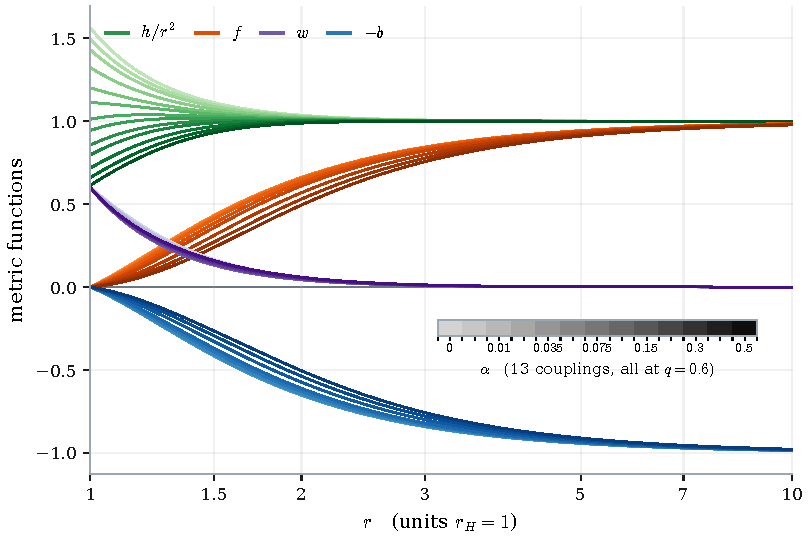
\includegraphics{figures/fig-profiles.pdf}
 \caption{The four metric functions of \eqref{eq:ansatz} at all
 $\Ncouplings$ couplings of table~\ref{tab:extremal}, all at the same spin
 $q=\Nstartspin$ and in units $r_H=1$. One colour per function, one shade per
 coupling, running from $\alpha=0$ (lightest) to $\alpha=1/2$ (darkest).
 Two conventions follow fig.~1 of \cite{Brihaye:2010wp} so that the two figures
 can be compared directly: $h$ is shown as $h/r^2$, which tends to unity at
 infinity whereas $h$ itself grows like $r^2$, and $b$ as $-b$, because $b$ and
 $f$ otherwise overlap over most of the range. The boundary conditions are
 visible rather than imposed on the plot: $b=f=0$ and $w=q$ at $r=r_H$, and
 $b,f,h/r^2\to1$, $w\to0$ as $r\to\infty$.}
 \label{fig:profiles}
\end{figure}

\subsection{An analytic example: the static limit}
\label{sec:static}

The static member is the Boulware--Deser solution \cite{Boulware:1985wk}.
In our conventions,
\begin{equation}
 M=\frac{3\pi}{8}(r_H^2+2\alpha),\qquad
 T=\frac{r_H}{2\pi(r_H^2+4\alpha)},\qquad
 S=\frac{\pi^2}{2}r_H^3+6\pi^2\alpha r_H.
 \label{eq:static}
\end{equation}
This example also illustrates, in closed form, the constraints in
\eqref{eq:psi}. Differentiating \eqref{eq:static} at fixed radius, the mass
derivative $M_\alpha=3\pi/4$ is positive, but the entropy is not held fixed:
it changes by $S_\alpha=6\pi^2r_H$. There is no spin term, so subtracting the
entropy contribution is all that \eqref{eq:psi} requires, and gives
\begin{equation}
 \Psi_{\rm static}
 =\frac{3\pi}{4}-T(6\pi^2r_H)
 =\frac{3\pi}{4}\frac{4\bar\alpha-3}{1+4\bar\alpha},
 \qquad \bar\alpha=\frac\alpha{r_H^2}.
 \label{eq:psistatic}
\end{equation}
In particular $\Psi_{\rm static}\to-9\pi/4$ as $\alpha\to0$.
The mass derivative at fixed radius and the derivative at fixed entropy
can have opposite signs; keeping the entropy fixed requires the radius
to change. Equation~\eqref{eq:psistatic} satisfies \eqref{eq:smarr}
identically at zero spin.

Applying the numerical procedure at zero spin for $\Nstaticcouplings$
couplings reproduces the analytic mass, temperature, entropy and
potential to worst relative deviations $\Nstaticmassworst$,
$\Nstatictempworst$, $\Nstaticentropyworst$ and $\Nstaticpsiworst$,
respectively. These are checks against an analytic solution at finite
coupling. The potential changes sign at $\bar\alpha=3/4$, or $x=3/5$,
on the static branch. That result alone does not fix the sign on
all rotating solutions beyond the range sampled here.

\subsection{The perturbative potential from the literature}
\label{sec:perturbative}

The $\alpha=0$ potential is known in closed form at every spin, and
\eqref{eq:psizero} below is neither a guess of ours nor a fit to our data: it
is transcribed from a perturbative free energy in the literature, with the two
steps of that transcription spelled out here.

The source is Wu and L\"u \cite{Wu:2024xnb}, who compute the
$\mathcal O(\alpha)$ correction to the thermodynamics of Myers--Perry black
holes in a general quadratic-curvature theory, at fixed temperature and
angular velocities, with the same $1/16\pi G$ action normalisation used in
\eqref{eq:action}. Their result applies to the Gauss--Bonnet term because the
Myers--Perry background is Ricci-flat: the $R^2$ and $R_{\mu\nu}R^{\mu\nu}$
terms of $\mathcal L_\GB$ contribute nothing at this order, so at first order
the coefficient of their $R_{\mu\nu\rho\sigma}R^{\mu\nu\rho\sigma}$ is our
$\alpha$.

The first step is thermodynamic. Define the Gibbs potential
$\mathcal G=M-TS-\sum_i\Omega_iJ_i$. The extended first law
\eqref{eq:firstlaw} gives
$\dd\mathcal G=-S\,\dd T-\sum_iJ_i\,\dd\Omega_i+\Psi\,\dd\alpha$, so the
coefficient of $\alpha$ in $\mathcal G$ at fixed $T$ and $\Omega_i$ is
$\Psi$ evaluated on the Einstein solution, which we call $\Psi_0$.
Equation~(33) of the arXiv version of \cite{Wu:2024xnb}, specialised to $D=5$
with equal rotation parameters $a_1=a_2=a$, is then
\begin{equation*}
 \Psi_0=\frac{\Delta\mathcal G}{\alpha}
 =-\frac{\pi}{4r_+^4}\bigl(a^4-14a^2r_+^2+9r_+^4\bigr),
\end{equation*}
with $r_+$ the Boyer--Lindquist horizon radius.
The second step is the change of radial coordinate already recorded in
\eqref{eq:qmp}, which turns this into a function of our spin label alone:
\begin{equation}
 \Psi_0(q)=-\frac\pi4\bigl(u^2-14u+9\bigr),\qquad
 u=\frac{a^2}{r_+^2}=\frac{q^2}{1-q^2}.
 \label{eq:psizero}
\end{equation}

Equation~\eqref{eq:psizero} interpolates between the two ends of the vacuum
family, and reproduces both independently known endpoint values although
neither was used to obtain it. At $u=0$ the solution is static, and
\eqref{eq:psizero} returns $-9\pi/4$, which is the $\alpha\to0$ limit of the
closed-form Boulware--Deser potential \eqref{eq:psistatic} obtained in
section~\ref{sec:static} from an entirely different calculation. At $u=1$,
which by \eqref{eq:qmp} is $q=1/\sqrt2$ and hence extremality, it returns
$\pi$, the linear-order slope in \eqref{eq:published} taken from
\cite{Ma:2020xwi}. Between them it changes sign once, at
$q=\Nperturbativezero$. This is the analytic reference against which the
numerical response is tested at zero coupling.

We evaluate the numerical response on the Myers--Perry background at
$\alpha=0$. It agrees with \eqref{eq:psizero} to at least
$\Noracledigits$ significant digits at $\Noraclegood$ of
$\Noracletotal$ sampled spins, with worst relative deviation
$\Noracleworst$. No extrapolation in the coupling is needed, although
the numerical response and charge extraction remain discretised.

\subsection{The potential across the family}

Figure~\ref{fig:potential} shows $\Psi$ against $t_H$ for the
$\Nmapcouplings$ couplings walked over the whole spin range.
Every plotted point is one accepted rotating solution, and both of its
coordinates are measured on that same solution: $\Psi$ from its own linear
response \eqref{eq:response}, and $t_H$ from its own $T$ and $M$ through
\eqref{eq:massvars}. Neither axis uses a static quantity. In particular
$t_H$ is not the static value $\sqrt{1+2\bar\alpha}/(1+4\bar\alpha)$ held
fixed along a curve; that value is the $q\to0$ \emph{limit} the curve runs
towards, and the closed-form static potential \eqref{eq:psistatic} is plotted
there as a cross so that the approach can be checked. The walks stop at a
small nonzero spin, so the crosses lie just beyond the right-hand end of the
curves rather than on them.
The curves are therefore sequences of rotating solutions at fixed coupling,
parametrised by spin, and not the static potential replotted.

On those sequences $\Psi$ is negative
near the static member and becomes positive towards extremality.
Thus increasing $\alpha$ lowers the mass at fixed $(S,J)$ in the former
region and raises it in the latter. The location of the sign change
depends on the coupling.

\begin{figure}[t]
 \centering
 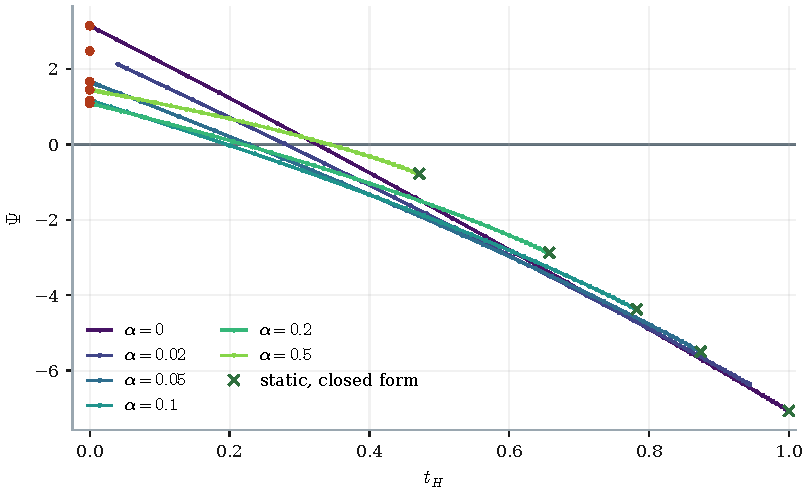
\includegraphics{figures/fig-potential.pdf}
 \caption{The measured potential along the $\Nmapcouplings$ stationary
 families that were walked over the whole spin range; the other
 $\Nnarrowcouplings$ couplings of table~\ref{tab:extremal} do not reach the
 low-spin end and are not shown. Each point on a curve is one rotating
 numerical solution, with $\Psi$ and $t_H$ both evaluated on that solution.
 A curve ends on the left at the coldest state reached and on the right at
 the slowest rotating state reached; the crosses are the exact static values
 \eqref{eq:psistatic}, plotted at the static temperature
 $t_H=\sqrt{1+2\bar\alpha}/(1+4\bar\alpha)$, which is the $q\to0$ limit each
 curve runs towards and not a point on it. Circles at $t_H=0$ are the
 extrapolated extremal values of table~\ref{tab:extremal}, intercepts of fits
 rather than constructed solutions.}
 \label{fig:potential}
\end{figure}

Every crossing in table~\ref{tab:locus} is bracketed by two accepted
solutions of opposite sign, and both endpoints of the bracket are given there.
The quoted position between them is an interpolant, so the digits it carries
are not the width of the bracket and should not be read as one. What they can
be calibrated against is the zero-coupling row, where the analytic zero
\eqref{eq:psizero} is known: the crossing is bracketed by solutions
$\Nlocuszerogap$ apart in $q$ and the interpolant lands $\Nlocuszerodev$ from
the analytic value, so the interpolation is better than the sampling by two
orders of magnitude, and it is that, rather than the bracket, that supports the
digits printed. In the scaled spin the locus moves from
$j=\Njlocusfirst$ to $\Njlocuslast$. In temperature it moves from
$t_H=\Ntlocusfirst$ down to $\Ntlocusmin$ at
$\alpha=\Nalphalocusmin$, then increases. A turning point in this
coordinate does not by itself establish a common physical mechanism
with the minimum of the extremal slope.

\begin{table}[t]
 \centering\small
 \begin{tabular}{@{}cccccc@{}}
 \toprule
 $\alpha$ & $x$ & $t_H$ & bracket width in $t_H$ & $j$ & $q$\\
 \midrule
 \Nlocustable
 \bottomrule
 \end{tabular}
 \caption{The measured sign-change locus, for the $\Nmapcouplings$ couplings
 whose walks cover the low-spin end where $\Psi$ is negative; at the other
 $\Nnarrowcouplings$ no crossing is bracketed by accepted solutions and none
 is reported. Digits of the interpolant are
 supplied for reproducibility, not as an error estimate. At $\alpha=0$
 the crossing is $q=\Nlocuszero$, compared with the analytic
 $q=\Nperturbativezero$.}
 \label{tab:locus}
\end{table}

\subsection{The extremal mass and its slope}
\label{sec:shift}

The walks reach $\tau\le\Ntaufloor$ at every coupling and $\Ntaubest$ at the
closest approach, in the scaled temperature $\tau$ of \eqref{eq:spinvars};
the value at each coupling is the $\tau_{\min}$ column of
table~\ref{tab:extremal}, which is the scaled temperature of the coldest
solution actually constructed there. The extrapolated branch is given in the
same table. Central values are the $T=0$ intercepts of cubic fits in the
unscaled temperature $T$ through the six coldest states at each coupling.

Every row of table~\ref{tab:extremal} is an extrapolation from positive
temperature, not a solution constructed at $T=0$: no state in the dataset has
zero temperature, and a row's temperature is zero by construction. What the
table reports instead is how far the extrapolation had to reach, the column
$\tau_{\min}$, which varies by orders of magnitude across the couplings; the
rows with the largest $\tau_{\min}$ carry the largest sensitivity. The entries
are therefore central extrapolants rather than measurements at extremality, and
the extrapolation is the one step of this calculation that no check in
section~\ref{sec:checks} repeats independently.

Figure~\ref{fig:extrapolation} shows that step itself, which a table of
intercepts hides. For each coupling it plots the six states the production fit
uses, the cubic fitted through them, the intercepts returned by the other
twenty fits of the sensitivity list, and the residuals the production fit
leaves. Three things are visible there. The fit describes its own points to
$\Nfitresidualworst$ or better at every coupling, which is small compared with
every sensitivity in table~\ref{tab:extremal}; so the envelope in that table is
not driven by a poor fit but by the length of the extrapolation. The
distance the fit travels differs by more than an order of magnitude between
couplings, and the four whose curves travel furthest are precisely the four
carrying the largest sensitivities in table~\ref{tab:extremal}. And the competing intercepts cluster at the axis rather
than scattering, so the spread the table reports is a spread between models
that mostly agree, not a disagreement about the value.

What the figure cannot show is a bias shared by all twenty-one fits. We have
not derived the leading near-extremal powers of $T$ for this system, so the
cubic is a convenience and not a model of the approach to extremality; the
square-root and logarithmic probes in table~\ref{tab:models} test for two
specific departures from analyticity and not for the general case. One further
stability test is reported in appendix~\ref{app:numerics}: refitting with each
of the six states removed in turn moves the intercept by at most
$\Nlooworst$, so no single cold or warm state carries the result.

The \emph{sensitivity} column answers one question: by how much does that
intercept move when the fit is changed? We refit the same states with
polynomials of degree one, two and three, on the six coldest states and on up
to the twelve coldest, in the coordinate $T$ and in the coordinate $\tau$, and
with two non-polynomial models; the quoted half-width is the largest
displacement of the intercept over that whole list. It measures sensitivity to
a stated set of modelling choices: it carries no confidence level, is not a
standard error, and cannot detect an error common to every fit in the list,
such as a systematic error in the underlying charges. Every band and spread
quoted below is of this kind. The full list is in
appendix~\ref{app:numerics}; the contribution of the two non-polynomial
models, which dominates the envelope at most couplings, is tabulated there in
table~\ref{tab:models}.

\begin{table}[t]
 \centering\small
 \begin{tabular}{@{}ccccccccc@{}}
 \toprule
 $\alpha$ & $y$ & $x$ & $\tau_{\min}$ & $\mu$ &
 $\Psi_\ext$ & sensitivity & $j$ & $\sigma$\\
 \midrule
 \Nextremaltable
 \bottomrule
 \end{tabular}
 \caption{The extrapolated extremal branch; these rows are $T=0$ intercepts
 of fits and not solutions, so the temperature of a row is zero by
 construction. What is reported instead is $\tau_{\min}=\min TJ^{1/3}$, the
 scaled temperature of the coldest solution the walk at that coupling actually
 reached. The sensitivity refers to $\Psi_\ext$ and to no other column; it is
 defined in section~\ref{sec:shift} and constructed in
 appendix~\ref{app:numerics}. The first row is compared with
 $\mu=(3/2)\pi^{1/3}$ and $\Psi_\ext=\pi$ in section~\ref{sec:checks}.}
 \label{tab:extremal}
\end{table}

\begin{figure}[t]
 \centering
 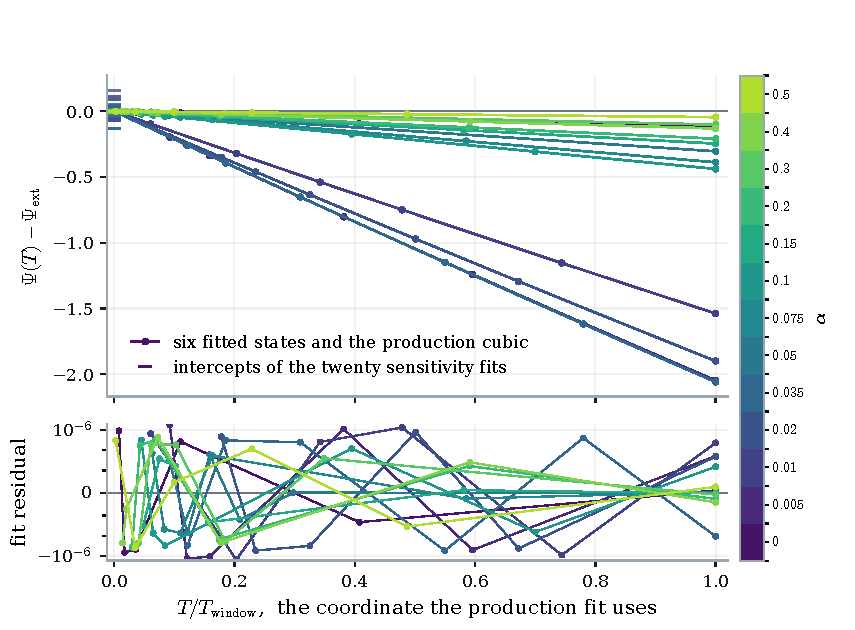
\includegraphics{figures/fig-extrapolation.pdf}
 \caption{The zero-temperature extrapolation, which produces every row of
 table~\ref{tab:extremal}. Filled circles are the $\Nfitwindow$ coldest
 accepted solutions at each coupling and the line through them is the
 production cubic; the abscissa is the temperature divided by the temperature
 of the warmest fitted state, the coordinate the fit itself uses, so that
 windows spanning four decades of $T$ can be compared, with the physical
 temperatures given by the $\tau_{\min}$ column of table~\ref{tab:extremal}.
 The central value is subtracted, so every curve reaches the origin by
 construction and the figure shows how far it travelled to get there. Short horizontal ticks on the left axis are
 the intercepts of the other twenty fits in the sensitivity list; the envelope
 of those ticks is the sensitivity column of table~\ref{tab:extremal}, and the
 lower panel gives the residuals of the production fit on a symmetric
 logarithmic scale.}
 \label{fig:extrapolation}
\end{figure}

The main qualitative result is visible in figure~\ref{fig:shift}:
the slope $\Psi_\ext$ is positive throughout the sampled range,
falls below its perturbative value, and subsequently increases.
The lowest sampled central value is $\Npsimin$ at $y=\Nymin$,
with fit sensitivity $\Ngriderror$. Its neighbouring samples lie at
$y=\Nminimumlow$ and $\Nminimumhigh$.
The last sampled value is $\Npsilast$ at $y=\Nylast$.
The suppression at the lowest sampled point relative to $\pi$ is
about a factor $\Nsuppression$.
We do not assign a precise location or confidence interval to a
continuous minimum between the sampled couplings.

The central extrapolated $M_\ext$ remains increasing at fixed $J$ across the
sampled range: the $\mu$ column of table~\ref{tab:extremal} is monotone, and
its increments exceed the corresponding spreads in table~\ref{tab:budget} by
two orders of magnitude or more. Those spreads, however, are the three degree
checks only. Given the same twenty-fit list as the potential
(appendix~\ref{app:numerics}), the envelope of $\mu$ at the smallest couplings
becomes comparable with the increments between neighbouring couplings. There
the increase of the extremal mass rests on the sign of $\Psi_\ext$, whose
envelope is far smaller than its value, rather than on the mass curve alone.
The accumulated mass change is the integral of the slope:
\begin{equation*}
 M_\ext(J,\alpha)-M_\ext(J,0)
 =J^{2/3}\int_0^{\alpha/J^{2/3}}\Psi_\ext(y')\,\dd y'.
\end{equation*}
Thus the suppression of the local slope is not a suppression factor
for the total mass shift.

Figure~\ref{fig:massext} shows the extremal mass itself. The plotted $\mu$ is
not this integral: it is formed at each coupling from the separately
extrapolated asymptotic charges, $\mu=M_\ext/J_\ext^{2/3}$, and the integral is
compared with it below. Across the sampled range $\mu$ rises by
$\Nmugrowth\%$, while the first-order
expression \eqref{eq:published} runs above it and overshoots by a factor
$\Nlinearratio$ at the largest coupling. The fall of the slope below $\pi$ is a
fall in the rate: the extremal mass grows more slowly than linear order
predicts, not more slowly than at $\alpha=0$. The right-hand panel places the
same branch in the $(x,j)$ plane of \cite{Kleihaus:2023zzs}, whose reported
domain of existence is bounded by $x<1$ and $j\le1$; our branch stays inside
both. Scale invariance ties the two panels, since $M_\ext=J^{2/3}\mu(y)$ gives
\begin{equation}
 j_\ext(y)=\biggl[\frac{\mu(0)}{\mu(y)}\biggr]^{3/2},
 \qquad \mu(0)=\tfrac32\pi^{1/3},
 \label{eq:jofmu}
\end{equation}
which our separately extrapolated $j$ and $\mu$ satisfy to
$\Njrelationworst$. The decrease of $j$ along the branch is therefore the
increase of $\mu$ re-expressed, and not an independent measurement.

\begin{figure}[t]
 \centering
 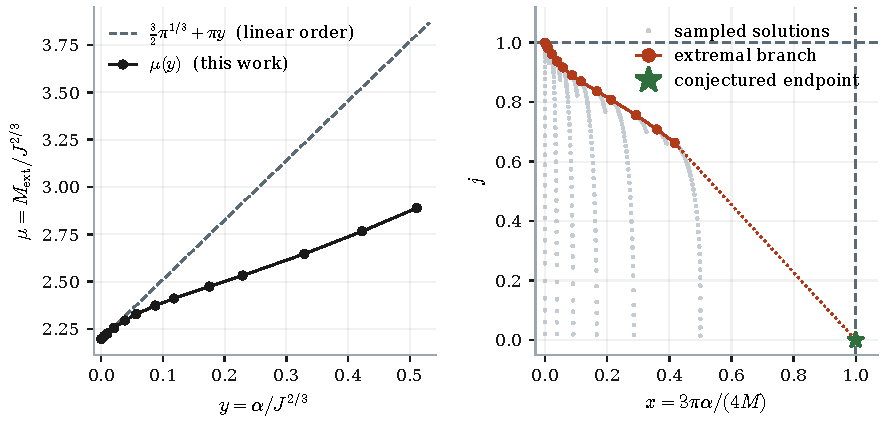
\includegraphics{figures/fig-massext.pdf}
 \caption{Left: the extremal mass in scale-invariant form,
 $\mu=M_\ext/J^{2/3}$ against $y=\alpha/J^{2/3}$, with the first-order line
 \eqref{eq:published} dashed. Right: the same branch in the $(x,j)$ plane of
 \cite{Kleihaus:2023zzs}, with every accepted non-extremal solution in grey,
 the bounds $x<1$ and $j\le1$ reported there dashed, and the endpoint conjectured
 there as a star; the dotted segment joins our last sampled point to that
 endpoint and is not computed. Every plotted extremal point is a $T=0$
 intercept of a fit and not a constructed solution; $\mu$ is formed from the
 extrapolated mass and angular momentum, not by integrating $\Psi_\ext$. The
 points carry no error bars. Their twenty-fit envelopes are discussed in
 appendix~\ref{app:numerics}, and the three-fit spreads in
 table~\ref{tab:budget}.}
 \label{fig:massext}
\end{figure}

We compare the potential with a second quantity formed from the
extrapolated masses and spins. Scale invariance implies
\begin{equation}
 \int_{y_1}^{y_2}\Psi_\ext(y)\,\dd y=\mu(y_2)-\mu(y_1).
 \label{eq:identity}
\end{equation}
The two sides reach the mass curve by different paths. The right side uses only
the mass and angular momentum read at infinity, along the extremal branch. The
left side also uses the temperature, the Wald entropy with its explicit
$\alpha$ term, the horizon angular velocity, the coupling derivatives of the
response solve and the assumption that $T\,\partial S_\ext/\partial\alpha$
vanishes at extremality, and it uses them along the fixed-$(r_H,\Omega_H)$
direction of \eqref{eq:psi}. Agreement therefore checks that the numerical
$(M,T,S,\Omega_H,J,\Psi)$ satisfy the extended first law consistently along
two different paths through the solutions: a wrong entropy term, temperature,
derivative or relative normalisation of $M$ and $S$ would each appear as a
mismatch. Since the extended first law is a theorem
\cite{Kastor:2010gq,Neri:2024}, this validates the numerics, not the law. It is
also not an independent determination of $M_\ext$. Both sides share the
solutions, the field equations and their discretisation, and the
zero-temperature extrapolation: $M$, $J$ and $\Psi$ are extrapolated
separately but with the same kind of fit through the same cold states, so a fit
that misses the true approach to extremality biases every intercept. Such a
bias need not cancel in \eqref{eq:identity}, but its effects on the two sides
can be correlated, and agreement does not bound them.

We integrate a local cubic interpolant through the four nearest
potential samples. The largest interval discrepancy in
\eqref{eq:identity} is $\Nrouteworst$, or $\Nrouteworstrel$
relative to the corresponding change in $\mu$.
Two different cumulative figures have to be distinguished. The discrepancy
accumulated across the whole range, that is its value at the last interval
$y=\Nroutecumulativey$, is $\Nroutecumulativeend$ on a total change
$\Nmutotal$; the largest \emph{running} value, reached before the last
interval and then partly cancelled, is $\Nroutecumulative$. Using trapezoids
instead gives a largest interval discrepancy $\Nroutetrapezoid$.
The comparison includes quadrature error and correlated errors
in the observables. Propagating the recorded extrapolation spreads of both
routes, the discrepancy is within the combined spread at
$\Nroutewithinspread$ of the $\Nrouteintervals$ intervals, the worst case
reaching $\Nroutespreadratio$ of it; since the two routes share those spreads
this is a consistency statement about the quadrature and not an independent
confirmation. The recorded spreads are the narrow ones: for $\mu$ the three
degree checks, and for $\Psi$ an earlier envelope narrower than that of
table~\ref{tab:extremal}. The twenty-fit envelopes of
appendix~\ref{app:numerics} are wider for both, so the count above is
conservative. Agreement of the changes in $\mu$ does not
bound a common offset in the masses, and we do not use it as an
absolute mass-accuracy estimate or a calibration of the sensitivity bars.

The same envelopes settle which route is the more precise. Interval by
interval, the potential determines the change in $\mu$ about an order of
magnitude more precisely than the difference of the extrapolated masses, at
every sampled interval; the open squares of figure~\ref{fig:shift} are the
noisier slope estimate, most of all at the smallest couplings, where the
spacing is finest and the walks are narrowest. Cumulatively the comparison
splits. Summed from $y=0$, the errors of $\Psi_\ext$ accumulate, and the
integrated slope is the better determination of $\mu$ only at the smallest
couplings; beyond them $\mu$ read at infinity is. Neither route escapes the
extrapolation in temperature: $\Psi_\ext$ is the more precise slope because it
extrapolates more stably than $M$ and $J$, not because it avoids that step.

\begin{figure}[t]
 \centering
 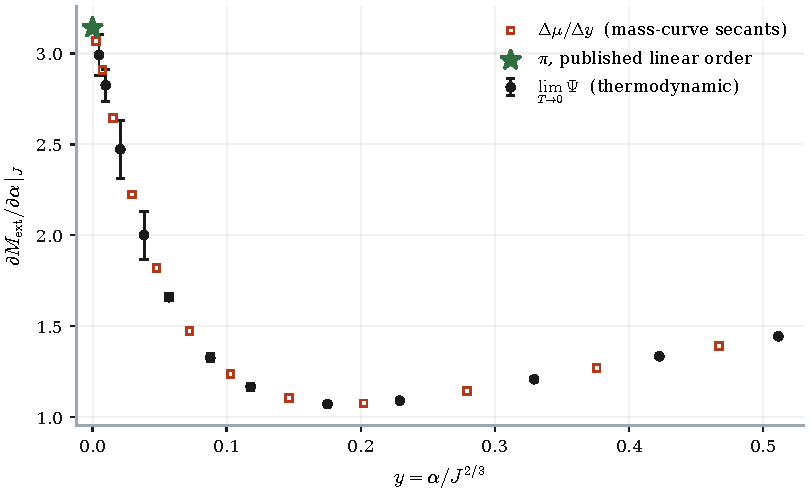
\includegraphics{figures/fig-shift.pdf}
 \caption{The extremal mass slope. Circles show the extrapolated potential
 with its fit-sensitivity envelope; open squares show secants of $\mu(y)$ at
 interval midpoints. A secant is an interval average rather than a pointwise
 derivative, and the two estimates share numerical inputs. The squares carry
 no error bars. Each inherits the $\mu$ envelopes of its two ends divided by
 the interval, which with the twenty-fit list is comparable with the secant
 itself at the smallest couplings and well above the envelope of $\Psi_\ext$
 everywhere (section~\ref{sec:shift}). The star is the
 perturbative value $\pi$ of \cite{Ma:2020xwi}, which is not imposed in
 the response calculation.}
 \label{fig:shift}
\end{figure}

A one-sided quadratic fit to the lowest-coupling mass samples gives
$\mu'(0)=\Nmassslope$, differing from $\pi$ by $\Nmassslopedev$.
Varying the number of samples gives a spread $\Nmassslopespread$.
This derivative uses the mass curve rather than the entropy formula,
but still relies on the thermodynamic extraction and extremal extrapolation.

\section{Checks against known results}
\label{sec:checks}

The analytic static and perturbative checks were described above.
Here we compare the extremal mass and entropy with results from the literature
and distinguish those comparisons from internal consistency tests.

\paragraph{Einstein and perturbative extremal limits.}
At $y=0$ we obtain
\begin{equation*}
 \mu=\Nmuzero,\qquad \tfrac32\pi^{1/3}=\Nmasscoefficient,\qquad
 \Psi_\ext=\Npsiextzero .
\end{equation*}
The absolute deviations from their respective analytic values are
$\Nmuzerodev$ and $\Npsiextzerodev$, respectively.
These numbers result from the same continuation and extrapolation
used at finite coupling; the limiting constants are not fitted constraints.
The agreement at $y=0$ does not by itself establish the error at finite $y$.

\paragraph{The potential from the Smarr relation.}
The response calculation of section~\ref{sec:response} is the one step of this
work with no analytic counterpart at finite coupling and finite spin, so it is
worth checking against something that does not use it. The Smarr relation
\eqref{eq:smarr} is such a thing. Read as an equation for $\Psi$ rather than as
a residual, it gives
\begin{equation}
 \Psi_{\rm Smarr}=\frac{2M-3TS-6\Omega_HJ}{2\alpha},
 \label{eq:psismarr}
\end{equation}
which involves only the charges of a single solution: no Jacobian, no linear
solve, no parameter derivative and no second solution. It is therefore a
genuine test of the implicit-response machinery --- of \eqref{eq:response}, of
the chain-rule assembly, of the complex-step parameter derivative and of the
explicit $\partial_\alpha$ of the entropy --- and not a repetition of it. What
it does share with the response is the set of solutions and the asymptotic
charge extraction, so a bias in either would move both.

Over the $\Nsmarrstates$ accepted states at $\alpha\ne0$, \eqref{eq:psismarr}
reproduces the response value to a worst relative difference
$\Nsmarrpsiworst$, worst absolute difference $\Nsmarrpsiabsolute$.
Extrapolating $\Psi_{\rm Smarr}$ to $T=0$ by the same cubic used for the
production values gives the comparison in table~\ref{tab:smarr}: the two routes
to $\Psi_\ext$ agree to $\Nsmarrextworst$ relative at all
$\Nsmarrextcouplings$ finite couplings, well below every fit sensitivity in
table~\ref{tab:extremal}. The division by
$\alpha$ in \eqref{eq:psismarr} is ill-conditioned as $\alpha\to0$, which is
why no row appears at $\alpha=0$; at $\alpha=0$ the corresponding test is the
perturbative potential of section~\ref{sec:perturbative}. At finite coupling
the Smarr route could supply $\Psi$ without the linear solve. The response
calculation earns its place where Smarr is weak, at small coupling, where the
numerator of \eqref{eq:psismarr} is a near-cancellation divided by a small
$\alpha$, and because it does not rely on the scaling argument. Smarr and the
subtraction \eqref{eq:psi} are the same first law taken along two directions,
the scaling direction and the coupling direction, so their agreement is one
consistency test of the numerics and not two.

\begin{table}[t]
 \centering\small
 \begin{tabular}{@{}cccc@{}}
 \toprule
 $\alpha$ & $\Psi_\ext$, response & $\Psi_\ext$, Smarr & relative difference\\
 \midrule
 \Nsmarrtable
 \bottomrule
 \end{tabular}
 \caption{The extremal potential by two routes. The first column repeats
 table~\ref{tab:extremal}; the second extrapolates \eqref{eq:psismarr},
 evaluated state by state from the charges alone, to $T=0$ with the same cubic
 through the same $\Nfitwindow$ states. The two share the solutions and the
 charge extraction but not the response solve. There is no $\alpha=0$ row
 because \eqref{eq:psismarr} divides by the coupling.}
 \label{tab:smarr}
\end{table}

\paragraph{The potential as an on-shell action.}
At fixed temperature and angular velocities the Gibbs potential of a stationary
black hole is its on-shell action per unit time, and the only \emph{explicit}
dependence of that action on $\alpha$ is the Gauss--Bonnet term of
\eqref{eq:action}. Differentiating at fixed $(T,\Omega_i)$ and discarding the
implicit variation with the field equations gives
\begin{equation}
 \Psi=-\frac1{16\pi}\int_\Sigma\dd^4x\,\sqrt{-g}\,\mathcal L_\GB ,
 \label{eq:onshell}
\end{equation}
with $\Sigma$ a stationary spatial slice outside the horizon; the integral
converges because $\mathcal L_\GB$ falls off like $r^{-8}$ on an
asymptotically flat solution while $\sqrt{-g}$ grows like $r^3$. The boundary
terms of the action carry $\alpha$ too, and that their net contribution to
\eqref{eq:onshell} vanishes for this family is part of what the test below
confirms. This route uses no Jacobian, no linear solve, no
parameter derivative and --- unlike \eqref{eq:psismarr} --- no asymptotic
charge extraction. It reads $\Psi$ off the curvature of the solution itself,
which is why it tests a different part of the chain than either of the two
checks above.

Evaluating the integrand with the same independent curvature evaluator that
gates acceptance, on the $\Nonshellstates$ archived spectral profiles,
reproduces the response value to a worst relative difference $\Nonshellworst$
and a worst absolute difference $\Nonshellabsolute$. The quadrature is
described in appendix~\ref{app:numerics}. Those states reach
$\alpha=\Nonshellalphahigh$ but only $q=\Nonshellspinhigh$: the near-extremal
states that carry the zero-temperature extrapolation are not among them, so
this check covers the potential across the coupling range and not at the
extremal end.

\paragraph{Extremal entropy.}
The near-horizon entropy function determines $S_\ext/J$ as a function of $y$
without integrating the radial equations. We rederived it rather than
transcribing it, as summarised in appendix~\ref{app:nearhorizon}, and checked
the rederivation against the equations of \cite{Brihaye:2010wp};
the curve in figure~\ref{fig:entropy} is that rederived solution and not a
quotation. Solving its algebraic equations numerically at finite coupling gives
the comparison shown there; the worst relative difference
from the extrapolated bulk entropy is $\Nhorizonworst$.
This validates the extremal entropy at finite coupling, but does not
provide a near-horizon measurement of the asymptotic mass.

\begin{figure}[t]
 \centering
 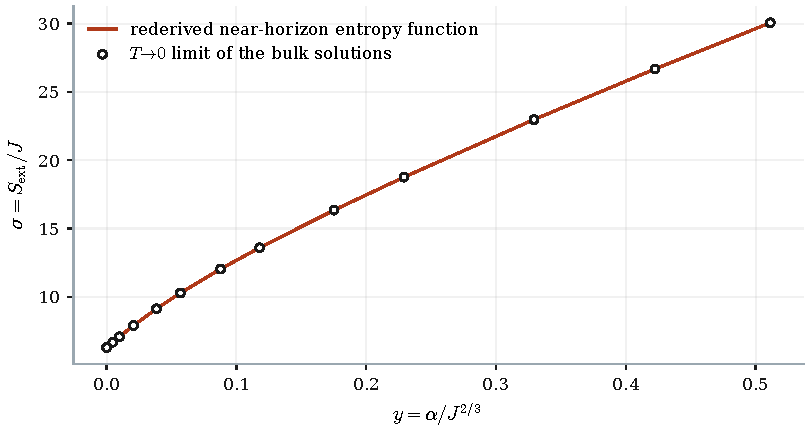
\includegraphics{figures/fig-entropy.pdf}
 \caption{Extremal entropy per angular momentum. The line joins values from
 our rederived near-horizon entropy function, checked against the equations of
 \cite{Brihaye:2010wp} to the precision quoted in the text; the points are
 extrapolations of bulk solutions to zero temperature.}
 \label{fig:entropy}
\end{figure}

In the variables of \cite{Brihaye:2010wp}, our near-horizon solutions
satisfy its eqs.~(4.11) and (4.12) to $\Npublishedstationarity$
and $\Npublishedspin$, respectively. This comparison checks the
coupling conversion $\alpha_{\rm ref.}=4\alpha$ of
table~\ref{tab:conventions}. One comparison with the same reference does not
close; it is discussed in section~\ref{sec:discussion}.

\paragraph{Internal thermodynamic checks.}
At $\Nconsistencypoints$ selected states we evaluate the first law
in the spin direction at fixed coupling:
\begin{equation*}
 \partial_q M-T\,\partial_q S-2\Omega_H\,\partial_q J=0.
\end{equation*}
Its worst residual is $\Nfirstlawworst$ relative to the largest term.
We also evaluate $-T\,\partial_\alpha S|_{M,J}$ using coupling and spin
responses and the scale direction. It agrees with $\Psi$ to
$\Ngoonpencoworst$ relative. This is an internal check constructed
from the same observables, not an independent test of the first law.
No degeneracy is implied by the static value $J=0$:
generically $J$ vanishes linearly with spin and its spin derivative
there is nonzero.


\section{Discussion}
\label{sec:discussion}

The observable calculated here is the response of mass to the Gauss--Bonnet
coupling at fixed entropy and angular momenta, and its zero-temperature limit
is the response of the extremal mass at fixed angular momenta, provided the
branch has a regular thermodynamic limit. Stated at the precision the evidence
supports: on the equal-spin branch continuously connected to five-dimensional
Myers--Perry, the positive-temperature solutions and their zero-temperature
extrapolations give a $\partial M_\ext/\partial\alpha|_J$ that is positive over
the sampled range, falling from the perturbative value $\pi$ to a broad low
region near $\Npsiminshort$ and rising again to $\Npsilastshort$. The positive
initial slope was already known; the fall and the subsequent rise are the
finite-coupling behaviour investigated here. Both moves exceed the fit
sensitivities of the rows involved by more than an order of magnitude. What
those sensitivities do not resolve is where the turning point lies between the
sampled couplings, which is why we quote a lowest sampled value rather than a
minimum.

Slope and accumulated mass change have to be kept apart. At fixed $J$ the
central extrapolated extremal mass increases throughout the range measured;
only its rate of increase turns over, reaching its lowest sampled value near
$\alpha=\Nalphamin$ in units $r_H=1$, corresponding to $x=\Nxmin$. By
$x=\Nhalfx$ the slope is already $\Nhalfpsi$, below half the perturbative
value. Outside this interval the data establish neither the sign nor the shape.

\subsection{Interpretation}
\label{sec:interpretation}

\paragraph{What a positive slope says.}
Two restatements make the sign concrete. The first concerns the spin bound:
by \eqref{eq:jofmu} a positive $\mu'$ is the same statement as a decreasing
$j_\ext$, so the largest spin a black hole of given mass can carry falls as the
coupling grows. The bound $j\le1$ reported in \cite{Kleihaus:2023zzs} is the
integrated form of the sign measured here pointwise. The second concerns the
horizon: setting $T=0$ in the Smarr relation \eqref{eq:smarr} gives
\begin{equation}
 \alpha\Psi_\ext=M_\ext-3\Omega_HJ ,
 \label{eq:smarrext}
\end{equation}
so $\Psi_\ext>0$ is exactly $M_\ext>3\Omega_HJ$, with the Gauss--Bonnet term
making up the difference between the extremal mass and the rotational term of
the Smarr relation. Both sides of \eqref{eq:smarrext} vanish at $\alpha=0$,
where extremal Myers--Perry satisfies $M_\ext=3\Omega_HJ$ exactly; the
first-order result $\Psi_\ext\to\pi$ of \cite{Ma:2020xwi} is then the statement
that the excess $M_\ext-3\Omega_HJ$ opens linearly in the coupling, and our
measurement is that it keeps opening, at a rate that falls and then recovers.

\paragraph{The sign of the potential.}
Equation~\eqref{eq:onshell} says what the sign of $\Psi$ is in terms of the
geometry: a positive $\Psi$ means the Gauss--Bonnet density integrated over the
exterior of a stationary slice is negative. The potential is negative near the
static, slowly rotating members of each family and positive towards
extremality, so the locus of table~\ref{tab:locus} is where that integrated
density changes sign, and $x=3/5$ on the static branch of
section~\ref{sec:static} is the same crossing at zero spin. The first law also
gives $\partial S/\partial\alpha|_{M,J}=-\Psi/T$, so the same sign says that a
negative integrated Gauss--Bonnet density is a decrease of entropy at fixed
mass and angular momenta. This is consistent with the entropy per spin along
the \emph{extremal} branch growing by a factor $\Nsigmagrowth$ over the sampled
range, because extremal states at fixed $J$ have different masses as $\alpha$
changes.

\paragraph{Where the slope is smallest.}
Dividing \eqref{eq:smarrext} by $J^{2/3}$, writing $\omega=\Omega_HJ^{1/3}$ for
the scale-invariant horizon angular velocity and using
$\Psi_\ext=\mu'$ gives
\begin{equation}
 3\omega(y)=\mu(y)-y\,\mu'(y),
 \qquad\text{hence}\qquad
 3\,\omega'(y)=-y\,\mu''(y).
 \label{eq:omegaidentity}
\end{equation}
For $y>0$ the extremal branch therefore has a stationary $\omega$ exactly where
the slope is stationary, and a minimum of $\mu'$ is a \emph{maximum} of
$\omega$: the inflection of the extremal mass is the extremal horizon with the
largest angular velocity in units of $J^{-1/3}$. That coupling is not otherwise
distinguished, and in particular is not a boundary of the domain of existence;
the sign-change locus of table~\ref{tab:locus} turns over at the neighbouring
sampled coupling $\alpha=\Nalphalocusmin$, and the grid does not resolve
whether the two coincide. Extrapolating $\omega$ on its own from the same walks
with the production model gives a maximum $\omega=\Nomegapeak$ at
$y=\Nomegapeaky$, the same sampled coupling at which $\Psi_\ext$ is smallest,
and satisfies \eqref{eq:omegaidentity} to $\Nomegaworst$ along the branch; at
$y=0$ it returns $\Nomegazero$ against the extremal Myers--Perry value
$\pi^{1/3}/2$, to $\Nomegazerodev$.

\paragraph{Why the slope has to rise again.}
The mass of a static Gauss--Bonnet black hole is bounded below by that of the
nakedly singular configuration, $M>3\pi\alpha/4$, and \cite{Kleihaus:2023zzs}
finds the same bound on the rotating solutions; in scale-invariant form it is
$\mu(y)>3\pi y/4$. Suppose the slope stayed below some $c<3\pi/4$ for all $y$.
Then $\mu(y)\le\mu(0)+cy$, which violates the bound once
$y>\mu(0)/(3\pi/4-c)$. The bound therefore forces $\mu'$ to return to at least
$3\pi/4=\Nslopeasymptote$, a value above every slope we measure, so the rise
from $\Npsiminshort$ to $\Npsilastshort$ over the upper part of our range is
required and not accidental. If in addition the extremal branch terminates as
conjectured in \cite{Kleihaus:2023zzs}, at $M=3\pi\alpha/4$ with $J\to0$, then
$\mu(y)/y\to3\pi/4$ and the average slope tends to $\Nslopeasymptote$, as does
$\mu'$ itself wherever it converges. Our sampled range stops well short of
that: the largest $x$ reached on the extremal branch is $\Nxextlast$, against
the conjectured endpoint at $x=1$. The measured rise is consistent with this
picture and does not establish it.

\paragraph{A constraint distinction at low spin.}
Holding the coordinate radius $r_H$ fixed does not hold the entropy fixed. At
$\alpha=1/2$ the measured mass initially decreases slightly with spin before
increasing, which the first law permits when the negative entropy contribution
exceeds the rotational one; the parity of $S(q)$ and $J(q)$ does not determine
the sign of $\partial_qM$. We therefore do not read a mass below the static
value at the same $r_H$ as an error, nor use that static value as a lower bound
on the rotating family. The bounds $x<1$ and $j\le1$ of
\cite{Kleihaus:2023zzs} are different statements: our largest scaled spin is
$\Nworstj$, and the extremal value falls to $\Njlast$ at the largest sampled
coupling.

\subsection{Limitations}

The leading limitation is the extremal extrapolation, and the displayed bands
measure sensitivity to specified fitting choices rather than numerical error.
Radial resolution is not the leading term: the complete ascending sequence and
its $T=0$ extrapolation were repeated at two coarser base resolutions at every
one of the $\Ncouplings$ couplings, including the three samples at
$y=\Nminimumlow$, $\Nymin$ and $\Nminimumhigh$ that bracket the turn in the
slope, and the extremal intercept moves by at most $\Nstudypsiworst$, below the
fit sensitivity at the same coupling in $\Nstudybelow$ of the $\Nstudywalks$
sequences. Appendix~\ref{app:numerics} reports that study observable by
observable and names the three reasons it bounds the resolution effect instead
of proving convergence; small field-equation residuals do not by themselves
bound the error in $M$, $J$, $S$ or $\Psi$, and what bounds it here is the
recomputation. The coupling coverage is incomplete and the spin coverage
uneven, the low-spin end and hence the sign-change locus being mapped at only
$\Nmapcouplings$ of the $\Ncouplings$ couplings, and the whole calculation is
restricted to equal spins. We do not show that the branch followed here is
unique, stable, or the lowest in mass among all five-dimensional solutions at
the same angular momenta, and we claim no global minimum mass anywhere. None of
the checks closes the gap that matters most:
the mass-curve comparison shares systematic errors with the potential, the
near-horizon route determines entropy rather than mass because the near-horizon
geometry discards the asymptotic normalisation, and the Smarr and on-shell
routes remove the response solve from the chain but not the solutions
themselves. Finally, the calculation treats Einstein--Gauss--Bonnet as a
classical theory with the action \eqref{eq:action}: second-order equations do
not by themselves establish existence, uniqueness, stability or well-posedness
at every coupling, and in a gravitational effective field theory terms beyond
Gauss--Bonnet contribute at the same order as the higher powers of $\alpha$
kept here, so the non-monotonic slope is not a universal prediction of a
derivative expansion. Causality restrictions on higher-curvature graviton
interactions are a further reason to separate this classical truncation from an
ultraviolet completion \cite{Camanho:2014apa}.

One comparison with \cite{Brihaye:2010wp} does not close. A separate
reconstruction of the non-extremal family gave an outer ergosurface radius
$1.102101$ against the $1.104$ quoted there, at $\alpha=1/2$ in our
convention. The discrepancy is unresolved and we do not offer it as evidence
of an erratum. It is also the only comparison of our rotating solutions at
finite coupling with values obtained numerically in \cite{Brihaye:2010wp}; the
comparisons that close are with closed-form statements or with the
near-horizon algebra, which does not use the bulk solver. It tests the reconstruction of the non-extremal metric
functions away from the horizon; it does not test the asymptotic charge
extraction, the response solve or the extrapolation, none of which uses the
ergosurface radius, and the near-horizon comparison of section~\ref{sec:checks},
which does test the coupling conversion, agrees to $\Npublishedstationarity$.

Four things would sharpen the result. A direct construction of extremal
solutions carrying their own response measurement, along the lines of
\cite{Kleihaus:2023zzs}, would remove the extrapolation, though built from
our field equations and charge extraction it would not be independent of
them; a derivation of the leading near-extremal powers of $T$ would do more
still, since it would replace the fitted cubic with a model; a second-order
perturbative calculation would test the initial departure from
$\Psi_\ext=\pi$ independently; and the extremal solutions of
\cite{Kleihaus:2023zzs} in tabulated form would test the mass curve
independently. The departures measured here are large enough that even a
percent-level comparison would test the sign of the shift and the overshoot
of the first-order formula, though not the slope.

\appendix
\section{Numerical construction and sensitivity analysis}
\label{app:numerics}

\paragraph{Radial discretisation.}
We set $r_H=1$, introduce $z=1/r$ and collocate in $\chi=1-z$.
The horizon is at $\chi=0$ and infinity at $\chi=1$.
The unknown amplitudes factor out the boundary behaviour:
\begin{equation*}
 b=(1-z^2)B,\qquad f=(1-z^2)F,\qquad
 h=\frac{1+z^4H}{z^2},\qquad w=z^4W.
\end{equation*}
They are represented at Chebyshev--Lobatto nodes.
At infinity, $\chi=1$, we impose $B=F=1$ and $H'=W'=0$, primes denoting
$\chi$-derivatives. At the horizon, $\chi=0$, where the solved interior
equations are singular, we impose three regularity relations together with
$W(\chi=0)=\Omega_H$, which is what fixes the spin of the solution.
The equations and horizon relations are generated symbolically.
Damped Newton iteration solves the collocation system.
Production walks use $N=\Nresolution$, with
$N=\Nrefinedresolution$ available when acceptance requires refinement;
$N=\Ncoarseresolution$ is used for selected comparison walks.

\paragraph{Jacobian and response.}
The production Newton and response solves use the same chain-rule
assembly of $\partial R_N/\partial u$. Local partial derivatives
are computed by complex step: seven vectorised partials of the
interior equations and nine of the horizon relations.
The coupling and angular-velocity derivatives are computed by
complex step in the respective parameter, with $\epsilon=10^{-20}$.
For a real analytic function,
$\operatorname{Im}f(p+i\epsilon)/\epsilon=f'(p)+\mathcal O(\epsilon^2)$, so a
small imaginary step gives the derivative without subtracting nearly equal real
numbers and without a step size to refine.
The rational residual is evaluated using complex arithmetic without
non-analytic operations on the perturbed variables.
The assembled Jacobian is checked entrywise against a dense
complex-step perturbation of every nodal unknown, including profiles
that do not solve the equations.
This checks the chain-rule assembly; both implementations still
use complex-step differentiation.

\paragraph{Continuation.}
Starting from Myers--Perry, we continue in coupling and spin.
The tangent predictor
$u+\Delta\alpha\,\partial_\alpha u+\Delta q\,\partial_q u$
provides the initial guess for each nonlinear solve.
In the tested near-extremal sequences it reaches states at which
reusing the previous solution failed to converge.
The predictor is only an initial guess: every retained state
must satisfy the same acceptance checks.

\paragraph{Acceptance and conditioning.}
An evaluator separate from the generated radial equations constructs
curvature tensors from the metric and checks
$G_{\mu\nu}+\alpha H_{\mu\nu}$ at $51$ off-grid points.
We divide the maximum absolute residual over these points by the
maximum reference scale over the same points. The reference scale is
the largest of the Einstein and Gauss--Bonnet tensor contributions
and the square root of the absolute Kretschmann invariant.
The relative threshold is $10^{-8}$; the absolute residual is
recorded as well. The largest relative residual over the accepted
states is $\Ntensorworst$, and the largest relative Smarr residual
is $\Nsmarrworst$. These residuals diagnose equation closure; they
are not bounds on the error of an extracted observable.

The largest condition number in the selected $\Nconsistencypoints$
checks is $\Nconditionworst$. It is $\|\mathsf A\|_2\,\|\mathsf A^{-1}\|_2$
for the assembled $\mathsf A=\partial R_N/\partial u$ in the collocation
variables $(B,F,H,W)$ at the Chebyshev--Lobatto nodes, with no row
equilibration and no rescaling of the unknowns; the quantity is therefore
tied to that choice of variables and is not comparable with a condition
number reported by a solver using different ones. Multiplying a condition
number by machine precision estimates possible error amplification, not the
number of correct digits in $\Psi$.
These selected checks do not bound conditioning at all
near-extremal states or at every resolution.

\paragraph{Asymptotic charge extraction.}
The coefficients in \eqref{eq:charges} are obtained by fitting
compactified amplitudes in $z^2$. The three windows and degrees are
\Ntailwindows. The first is the production choice; the other two
measure sensitivity to that choice. We also compare masses
extracted from the $b$ and $f$ asymptotics.
The largest recorded relative diagnostic is $\Ntailspreadworst$.
All these extractions can share a bias, so a small spread does not
certify their absolute accuracy.
At $\alpha=0$, comparison with the analytic
$M=3\pi r_H^2/[8(1-q^2)]$ gives a worst relative deviation
$\Nvacuummassworst$ through $q=\Nvacuumspin$.
The static finite-coupling comparison is in section~\ref{sec:static}.
We have no corresponding analytic rotating mass at finite coupling.

\paragraph{The on-shell integral.}
Equation~\eqref{eq:onshell} is evaluated on the archived spectral profiles,
using the same independent curvature evaluator as the acceptance gate. On the
ansatz \eqref{eq:ansatz} the integrand factorises as
$\sqrt{-g}\,\mathcal L_\GB=\sin\theta\cos\theta\,D(r)$, which the run checks at
four polar angles rather than assuming; the angular integral is then $2\pi^2$
and $\Psi=-(\pi/8)\int_{r_H}^{\infty}D\,\dd r$. The radial integral uses
Gauss--Legendre quadrature in the compactified coordinate $\chi=1-1/r$ with
$\Nonshellnodes$ nodes. It cannot be refined indefinitely: $\mathcal L_\GB$ is
a difference of curvature squares that cancels to $\mathcal O(r^{-8})$, so
nodes pushed towards $\chi=1$ lose the density to floating-point cancellation
while $\dd r/\dd\chi$ amplifies what survives. The node count is therefore a
recorded parameter and the convergence ladder is stored with the result.

\paragraph{Central extrapolation.}
At each coupling, states are sorted by the physical temperature $T$
in units $r_H=1$. The central estimates of $M,J,S,\Psi$ are the
intercepts of cubic fits through the six coldest states.
The original degree checks use linear, quadratic and cubic fits
through four, five and six states, respectively.
The invariants $y,\mu,\sigma$ are then formed from the extrapolated
charges. The use of unscaled $T$ here is distinct from the use
of $\tau=TJ^{1/3}$ to report the distance to extremality.

\paragraph{Fit-sensitivity envelopes.}
For the potential we recompute fits on the six coldest states and
on up to twelve coldest states, using both $T$ and $\tau$.
For each coordinate and window we use polynomials of degree one,
two and three and the forms
\begin{equation*}
 c_0+c_1v+c_{1/2}\sqrt v,\qquad
 c_0+c_1v+c_2v^2+c_{\log}v^2\log v,
\end{equation*}
where $v$ is the chosen coordinate divided by its largest value
in the fitting window. This rescaling improves conditioning.
The half-width displayed in table~\ref{tab:extremal} and
figure~\ref{fig:shift} is the largest deviation of any of these
intercepts from the production central estimate, or the original
degree spread if larger.
The central values are unchanged by this reanalysis.

The tables apply this list to the potential only. Applied unchanged to $M$ and
$J$, pairing them fit by fit so that their correlation is kept and forming
$\mu$ from each pair, it widens the envelope of $\mu$ over the degree spread of
table~\ref{tab:budget} by up to several orders of magnitude, most where that
spread is smallest. This is the comparison on equal footing used in
section~\ref{sec:shift}: with the same fits on both sides, the potential is the
more precise slope in every sampled interval, and the integrated potential is
the more precise mass curve only at the smallest couplings. Whether the shifts
of the two routes across the twenty fits are correlated has not been
computed.

Table~\ref{tab:models} shows the largest changes from the square-root
and logarithmic models across the two coordinates and windows.
These terms are sensitivity probes, not a derivation of the
near-extremal expansion. Small changes for a given probe do not
exclude other non-analytic behaviour.
The envelope also includes the polynomial window and coordinate changes.

\begin{table}[t]
 \centering\small
 \begin{tabular}{@{}ccccc@{}}
 \toprule
 $\alpha$ & $T_{\min}$ & $T_{\max}/T_{\min}$ &
 square-root shift & logarithmic shift\\
 \midrule
 \Nmodeltable
 \bottomrule
 \end{tabular}
 \caption{Sensitivity of the potential intercept to non-polynomial
 fit models. $T_{\min}$ is the unscaled temperature of the coldest state at
 that coupling, and is the same state whose scaled temperature appears as
 $\tau_{\min}$ in table~\ref{tab:extremal}; the ratio column gives the span of
 the up-to-twelve-point window, which is the lever arm of the fit. Each shift
 is the largest absolute difference from the production central value over
 both windows and both coordinates. These two columns are part of the
 sensitivity envelope of table~\ref{tab:extremal}, not a separate estimate.}
 \label{tab:models}
\end{table}

\paragraph{Removing a fitted state.}
The envelope above varies the model, the window and the coordinate but always
fits the same states. A separate test varies the states: we refit the
production cubic $\Nfitwindow$ times, each time with one of the six fitted
states removed, keeping the model fixed so that only one thing changes. Five
points still over-determine a cubic. The largest resulting displacement of the
intercept over all couplings is $\Nlooworst$, and the largest residual the
production fit leaves on its own points is $\Nfitresidualworst$; both are
smaller than every sensitivity in table~\ref{tab:extremal}. Neither is a bound
on a bias shared by the six states, which is what a systematic error in the
underlying charges would be.

\paragraph{The uncertainty budget.}
Table~\ref{tab:extremal} carries a sensitivity for $\Psi_\ext$ alone, but $y$,
$\mu$, $j$ and $\sigma$ are extrapolated too, and the mass-curve check of
\eqref{eq:identity} depends on $y$ and $\mu$ directly. Table~\ref{tab:budget}
collects what is recorded for each. The spreads for $y$, $\mu$ and $\sigma$ are
those of their own intercepts across the original degree checks; the spread for
$j$ is obtained by forming $j$ from each pair of extrapolated $(M,J)$
intercepts, which propagates their correlation rather than adding them in
quadrature. The last two columns are the fit diagnostics of the preceding
paragraph.

These are not a combined error bound and are not to be added. The effects they
do not separate are radial resolution, which is measured at only
$\Ncontrastcouplings$ couplings (table~\ref{tab:contrast}); the asymptotic tail
extraction, whose recorded spread is $\Ntailspreadworst$ and which can be
biased without spreading; the nonlinear solver tolerance; the response linear
solve; and the interpolation used in \eqref{eq:identity}. Read as one number
per row, the $\Psi_\ext$ sensitivity is the largest of the effects we can
measure and not a bound on their sum.

\begin{table}[t]
 \centering\footnotesize\tightcolumns
 \begin{tabular}{@{}cccccccc@{}}
 \toprule
 $\alpha$ & $\delta y$ & $\delta\mu$ & $\delta j$ & $\delta\sigma$ &
 $\delta\Psi_\ext$ & fit residual & drop-one shift \\
 \midrule
 \Nbudgettable
 \bottomrule
 \end{tabular}
 \caption{What is recorded for every extrapolated column of
 table~\ref{tab:extremal}, not only for $\Psi_\ext$. The first four are
 intercept spreads across the original degree checks, $\delta j$ propagated
 through the extrapolated $M$ and $J$ together; $\delta\Psi_\ext$ is the
 envelope of table~\ref{tab:extremal}. The two kinds are not comparable: the
 degree spreads cover three fits and the envelope twenty, and the same twenty
 fits widen $\delta\mu$ considerably (appendix~\ref{app:numerics}). The last two columns are the largest
 residual the production cubic leaves on its own six states and the largest
 displacement of its intercept when one of those states is removed; they are
 not independent contributions to be combined.}
 \label{tab:budget}
\end{table}

\paragraph{Radial resolution.}
Production walks use $N=\Nresolution$, raised to $\Nrefinedresolution$ when a
state is refused. To bound what that choice costs, the complete ascending walk
and the complete $T=0$ extrapolation were repeated at $N=\Nstudyresolutions$ at
every one of the $\Nstudycouplings$ couplings: $\Nstudywalks$ independent
sequences, each using the production start spin, the production acceptance gates
and the production escalation rule, so that the base resolution is the only
thing varied. Only the ascending branch is walked, since the twelve coldest
states that enter the fit all lie on it. Table~\ref{tab:resolution} gives the
outcome observable by observable, because a small change in $\Psi_\ext$ does not
by itself bound a change in $M$, $J$, $S$, $y$ or $\mu$, and
\eqref{eq:identity} uses the last two.

Across all $\Nstudywalks$ sequences the extremal intercept moves by at most
$\Nstudypsiworst$ in $\Psi_\ext$, $\Nstudymuworst$ in $\mu$ and
$\Nstudyyworst$ in $y$, and the
extrapolated charges by at most $\Nstudymassworst$, $\Nstudymomentumworst$ and
$\Nstudyentropyworst$ relative in $M$, $J$ and $S$ respectively; the two
remaining columns of table~\ref{tab:budget} move by at most $\Nstudyspinworst$
in $j$ and $\Nstudysigmaworst$ in $\sigma$. The quantity
this has to be compared with is the fit sensitivity already quoted at the same
coupling. Figure~\ref{fig:resolution} draws the two together: at
$\Nstudybelow$ of the $\Nstudywalks$ sequences the resolution difference is
below that sensitivity, the worst ratio between them being $\Nstudyratio$.
Radial resolution is therefore not the leading term in the budget of
table~\ref{tab:budget}; the extrapolation is, by several orders of magnitude.
Raising the coarse resolution from $N=\Nstudylowresolution$ to
$N=\Nstudyhighresolution$ reduces the difference in $\Psi_\ext$ at
$\Nstudyshrink$ of the $\Nstudycouplings$ couplings.

Three things keep this short of a convergence proof. First, the escalation rule
means the
coldest states can be accepted at $N=\Nrefinedresolution$ on both sides; that
happens at $\Nstudyescalated$ of the $\Nstudywalks$ sequences, where the
comparison is weaker than the two base resolutions suggest. Second, a coarse
walk need not reach as cold as the production one, so the two fits can
extrapolate from different distances and the difference between them is not
purely a resolution effect; refitting both sides over a common temperature range
isolates the resolution and leaves a worst difference $\Nstudymatchedworst$ over
the $\Nstudymatchedwalks$ sequences in which both sides keep a full window.
Third, the shipped measurement was produced under \Nstudyshipped\ and this study
runs under \Nstudyhere, so each difference above bounds the change of resolution
and the change of environment together. Re-walking at the production resolution
here, at \Nstudycontrollist, attributes at most $\Nstudycontrolworst$ to the
environment alone. That is not a negligible share: at two of the three control
couplings it exceeds at least one of the two resolution differences measured at
the same coupling, and at $\alpha=1/2$ it exceeds both. The entries of
table~\ref{tab:resolution} are therefore upper bounds on the effect of the
resolution, not estimates of it, and the true resolution sensitivity of this
calculation is smaller than the table says. Table~\ref{tab:contrast} is free of that caveat: its two sides
were both computed in the shipped environment, at the $\Ncontrastcouplings$
couplings where that comparison exists, and there the extrapolated potential
moves by at most $\Ncontrastworst$ and $\mu$ by at most $\Ncontrastmu$.

\begin{table}[t]
 \centering\footnotesize\tightcolumns
 \begin{tabular}{@{}cccccccc@{}}
 \toprule
 $\alpha$ & $N$ & $\delta M/M$ & $\delta J/J$ & $\delta S/S$ &
 $\delta\Psi_\ext$ & $\delta y$ & $\delta\mu$ \\
 \midrule
 \Nresolutiontable
 \bottomrule
 \end{tabular}
 \caption{The radial-resolution study: the complete ascending walk and the
 complete $T=0$ extrapolation, repeated at two coarser base resolutions at every
 coupling. Each entry is the difference between the production value at
 $N=\Nresolution$ and the value the coarser sequence extrapolates to; the two
 sequences are independent from the first continuation step onwards. $M$, $J$
 and $S$ are quoted relative and the rest absolute, matching how each is used in
 the text. The columns are separate because they are separate: none of them
 bounds another.}
 \label{tab:resolution}
\end{table}

\begin{figure}[t]
 \centering
 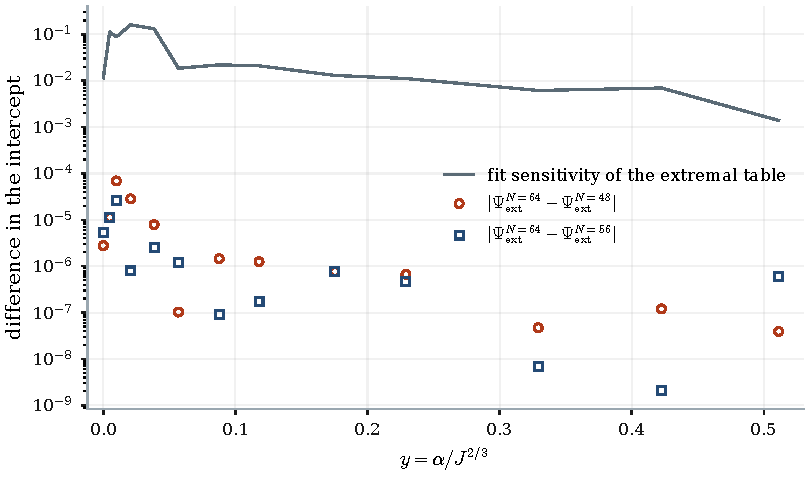
\includegraphics{figures/fig-resolution.pdf}
 \caption{The resolution study against the quantity it has to be compared with.
 Markers are the change in the extremal intercept when the whole sequence is
 recomputed at a coarser base resolution; the line is the fit sensitivity
 already quoted for the same coupling in table~\ref{tab:extremal}. The gap
 between them is the statement: at every coupling the extrapolation model
 dominates the radial resolution. The vertical scale is logarithmic and the two
 marker sets are the two coarse resolutions of table~\ref{tab:resolution}.}
 \label{fig:resolution}
\end{figure}

\begin{table}[t]
 \centering\small
 \begin{tabular}{@{}cccccc@{}}
 \toprule
 $\alpha$ & $\Psi_\ext$ at $N=\Nresolution$ & change at $N=\Ncoarseresolution$
 & $\mu$ at $N=\Nresolution$ & change & change in $y$ \\
 \midrule
 \Ncontrasttable
 \bottomrule
 \end{tabular}
 \caption{The resolution comparison recorded with the shipped measurement, at
 the $\Ncontrastcouplings$ couplings where it exists. It carries less coverage
 than table~\ref{tab:resolution} and one advantage over it: both sides were
 computed in the same environment, so these differences are attributable to the
 resolution alone.}
 \label{tab:contrast}
\end{table}

The integral comparison in \eqref{eq:identity} has its own
interpolation error and correlations with both sets of estimates;
we report its discrepancy separately instead of interpreting it as
coverage by independent error bars.

\paragraph{The profile atlas.}
Figure~\ref{fig:profiles} is produced by a separate run, whose only purpose is
to exhibit the solutions behind the rest of the paper and to test them along a
second route. It fixes $q=\Nstartspin$, climbs the spin from the vacuum in
steps of that size, and then climbs the coupling at fixed spin, seeding each
Newton solve with the previous solution and using no response predictor. The
production walks do the opposite: they climb the coupling first, with a
predictor, and then descend or ascend in spin. The two routes visit the same
$\Ncouplings$ solutions and agree on $M$, $J$, $S$ and $T$ to
$\Nprofileagreement$ relative. Each state in the atlas passes the same
boundary and independent tensor-residual gates as the production states, and
the run also checks that the vacuum member reproduces the closed-form
Myers--Perry horizon squashing $1/(1-q^2)$ and that $w(r_H)=\Omega_H$ is
recovered to machine precision.

\paragraph{Data and code.}
The supplementary table contains the $\Nstates$ accepted states,
their observables and acceptance diagnostics, one row per solution, so that
every point of figure~\ref{fig:potential} and every row of
tables~\ref{tab:locus} and \ref{tab:extremal} can be traced to the state it
came from. The radial amplitudes of figure~\ref{fig:profiles} are stored
separately, on the common grid used to draw them, and the fitted points,
residuals, competing intercepts and drop-one shifts behind
figure~\ref{fig:extrapolation} and tables~\ref{tab:models} and
\ref{tab:budget} are exported with them. The radial-resolution study is a
separate artifact carrying every state of all $\Nstudywalks$ coarse sequences,
so that table~\ref{tab:resolution} and figure~\ref{fig:resolution} can be
recomputed without repeating the solves.
The accompanying source tree contains the solver, symbolic
derivation scripts, tests and figure-generation script.
The latter also exports the fitted intercepts and sensitivity
envelopes used in this version, together with source hashes.

Every number in this manuscript is generated from the recorded measurement by
that script and none is typed into the source, so the PDF, the figures, the
tables and the data cannot disagree with one another: rebuilding reproduces
them or fails. What this arrangement does not by itself provide is an
immutable identifier for the state it was built from.
These materials document the calculation; this manuscript does
not claim an existing public archival DOI.

\section{The near-horizon entropy function}
\label{app:nearhorizon}
%======================================================================

The comparison in section~\ref{sec:checks} uses the extremal entropy obtained
from the near-horizon geometry, following section 4.2 of \cite{Brihaye:2010wp}.
We summarise our rederivation, which is independent of that reference in
execution though not in content.

For equal angular momenta the extremal near-horizon geometry is homogeneous,
with isometry group $SO(2,1)\times SU(2)\times U(1)$; see \cite{Kunduri:2013gce}
for the general classification of such geometries. It can be written in terms of
the $SU(2)$ invariant one-forms $\sigma_{i}$ as
\begin{equation}
  \dd s^{2} = v_{1}\Bigl(-r^{2}\dd t^{2} + \frac{\dd r^{2}}{r^{2}}\Bigr)
  + \frac{v_{2}}{4}\bigl(\sigma_{1}^{2}+\sigma_{2}^{2}\bigr)
  + \frac{v_{3}}{4}\bigl(\sigma_{3} + k\,r\,\dd t\bigr)^{2},
  \label{eq:nearhorizon}
\end{equation}
with $v_{1,2,3}$ and $k$ constants. On \eqref{eq:nearhorizon} both $R$ and
$\mathcal{L}_\GB$ are constant, and Sen's entropy function \cite{Sen:2007qy}
reduces the problem to algebra: with
\begin{equation}
  f(v,k) = \int \dd\theta\,\dd\varphi\,\dd\psi\,\sqrt{-g}\,
  \frac{R+\alpha\mathcal{L}_\GB}{16\pi}
  = \frac{\pi}{8}\,v_{1}v_{2}\sqrt{v_{3}}\,
  \bigl(R+\alpha\mathcal{L}_\GB\bigr),
\end{equation}
the equations of motion are $\partial f/\partial v_{i}=0$, the angular momentum
is $J=\partial f/\partial k$, and the entropy is the Legendre transform
$S_\ext = 2\pi\bigl(kJ-f\bigr)$ evaluated at the extremum.

We derived $R$ and $\mathcal{L}_\GB$ on \eqref{eq:nearhorizon} symbolically and
checked them against the same numerical curvature evaluator used for acceptance;
we then verified that the extremal solution satisfies the full field equations
$G_{\mu\nu}+\alpha H_{\mu\nu}=0$ component by component, since extremising a
reduced functional and solving the equations are not the same statement. At
$\alpha=0$ the system solves exactly, $k=1$, $v_{2}=4v_{1}$, $v_{3}=8v_{1}$,
giving $S_\ext = 2\pi J$, which is extremal Myers--Perry
($S=2\pi^{2}a^{3}$, $J=\pi a^{3}$ at $r_{+}=a$) with nothing tuned: the
$1/16\pi G$ of the action and the $2\pi$ of the Legendre transform were both
fixed beforehand. At finite coupling the branch is a root of an explicit
polynomial system, and it reproduces eqs.~(4.11) and (4.12) of
\cite{Brihaye:2010wp} to the precision quoted in section~\ref{sec:checks}.

Under $v_{i}\to\lambda v_{i}$, $\alpha\to\lambda\alpha$ both $J$ and $S_\ext$
scale as $\lambda^{3/2}$, so $\sigma=S_\ext/J$ and $y=\alpha/J^{2/3}$ are
invariant and are what figure~\ref{fig:entropy} compares. We emphasise that this
appendix produces no mass: the near-horizon geometry of an extremal black hole
determines its entropy as a function of its charges and no more, a point made in
\cite{Brihaye:2010wp} itself, where the absence of the corresponding $E(J)$
diagram is noted as an open problem.

%======================================================================
\begin{thebibliography}{99}
\bibitem{Ma:2020xwi}
  L.~Ma, Y.-Z.~Li and H.~L\"u,
  \emph{$D=5$ rotating black holes in Einstein-Gauss-Bonnet gravity: mass and
  angular momentum in extremality},
  JHEP \textbf{01} (2021) 201
  [\href{https://arxiv.org/abs/2009.00015}{arXiv:2009.00015}].
\bibitem{Kleihaus:2023zzs}
  B.~Kleihaus, J.~Kunz and E.~Radu,
  \emph{Phases of rotating black objects in $d=5$ Einstein-Gauss-Bonnet theory},
  Universe \textbf{9} (2023) 156
  [\href{https://arxiv.org/abs/2303.12471}{arXiv:2303.12471}].
\bibitem{Myers:1986un}
  R.~C.~Myers and M.~J.~Perry,
  \emph{Black holes in higher dimensional space-times},
  Annals Phys.\ \textbf{172} (1986) 304.
\bibitem{ArkaniHamed:2006dz}
  N.~Arkani-Hamed, L.~Motl, A.~Nicolis and C.~Vafa,
  \emph{The string landscape, black holes and gravity as the weakest force},
  JHEP \textbf{06} (2007) 060 [\href{https://arxiv.org/abs/hep-th/0601001}{hep-th/0601001}].
\bibitem{Kats:2006xp}
  Y.~Kats, L.~Motl and M.~Padi,
  \emph{Higher-order corrections to mass-charge relation of extremal black holes},
  JHEP \textbf{12} (2007) 068 [\href{https://arxiv.org/abs/hep-th/0606100}{hep-th/0606100}].
\bibitem{Goon:2019faz}
  G.~Goon and R.~Penco,
  \emph{Universal relation between corrections to entropy and extremality},
  Phys.\ Rev.\ Lett.\ \textbf{124} (2020) 101103
  [\href{https://arxiv.org/abs/1909.05254}{arXiv:1909.05254}].
\bibitem{Lovelock:1971yv}
  D.~Lovelock,
  \emph{The Einstein tensor and its generalizations},
  J.\ Math.\ Phys.\ \textbf{12} (1971) 498.
\bibitem{Reall:2019sah}
  H.~S.~Reall and J.~E.~Santos,
  \emph{Higher derivative corrections to Kerr black hole thermodynamics},
  JHEP \textbf{04} (2019) 021
  [\href{https://arxiv.org/abs/1901.11535}{arXiv:1901.11535}].
\bibitem{Wu:2024xnb}
  P.-Y.~Wu and H.~L\"u,
  \emph{Quadratic curvature correction and its breakdown to thermodynamics of
  rotating black holes},
  Phys.\ Rev.\ D \textbf{111} (2025) 104026
  [\href{https://arxiv.org/abs/2405.04576}{arXiv:2405.04576}].
\bibitem{Ma:2025qcf}
  L.~Ma and H.~L\"u,
  \emph{Quadratic curvature correction to 5D Myers-Perry metric},
  JHEP \textbf{05} (2026) 081
  [\href{https://arxiv.org/abs/2512.23797}{arXiv:2512.23797}].
\bibitem{Brihaye:2010wp}
  Y.~Brihaye, B.~Kleihaus, J.~Kunz and E.~Radu,
  \emph{Rotating black holes with equal-magnitude angular momenta in $d=5$
  Einstein-Gauss-Bonnet theory},
  JHEP \textbf{11} (2010) 098
  [\href{https://arxiv.org/abs/1010.0860}{arXiv:1010.0860}].
\bibitem{Sen:2007qy}
  A.~Sen,
  \emph{Black hole entropy function, attractors and precision counting of
  microstates},
  Gen.\ Rel.\ Grav.\ \textbf{40} (2008) 2249
  [\href{https://arxiv.org/abs/0708.1270}{arXiv:0708.1270}].
\bibitem{Kastor:2010gq}
  D.~Kastor, S.~Ray and J.~Traschen,
  \emph{Smarr formula and an extended first law for Lovelock gravity},
  Class.\ Quant.\ Grav.\ \textbf{27} (2010) 235014
  [\href{https://arxiv.org/abs/1005.5053}{arXiv:1005.5053}].
\bibitem{Neri:2024}
  G.~Neri and S.~Liberati,
  \emph{Covariant phase space analysis of Lanczos--Lovelock gravity with boundaries},
  [\href{https://arxiv.org/abs/2404.16981}{arXiv:2404.16981}].
\bibitem{Wald:1993nt}
  R.~M.~Wald,
  \emph{Black hole entropy is the Noether charge},
  Phys.\ Rev.\ D \textbf{48} (1993) R3427
  [\href{https://arxiv.org/abs/gr-qc/9307038}{gr-qc/9307038}].
\bibitem{Iyer:1994ys}
  V.~Iyer and R.~M.~Wald,
  \emph{Some properties of Noether charge and a proposal for dynamical black
  hole entropy},
  Phys.\ Rev.\ D \textbf{50} (1994) 846
  [\href{https://arxiv.org/abs/gr-qc/9403028}{gr-qc/9403028}].
\bibitem{Jacobson:1993xs}
  T.~Jacobson and R.~C.~Myers,
  \emph{Black hole entropy and higher curvature interactions},
  Phys.\ Rev.\ Lett.\ \textbf{70} (1993) 3684
  [\href{https://arxiv.org/abs/hep-th/9305016}{hep-th/9305016}].
\bibitem{Boulware:1985wk}
  D.~G.~Boulware and S.~Deser,
  \emph{String generated gravity models},
  Phys.\ Rev.\ Lett.\ \textbf{55} (1985) 2656.
\bibitem{Camanho:2014apa}
  X.~O.~Camanho, J.~D.~Edelstein, J.~Maldacena and A.~Zhiboedov,
  \emph{Causality constraints on corrections to the graviton three-point
  coupling},
  JHEP \textbf{02} (2016) 020
  [\href{https://arxiv.org/abs/1407.5597}{arXiv:1407.5597}].
\bibitem{Kunduri:2013gce}
  H.~K.~Kunduri and J.~Lucietti,
  \emph{Classification of near-horizon geometries of extremal black holes},
  Living Rev.\ Rel.\ \textbf{16} (2013) 8
  [\href{https://arxiv.org/abs/1306.2517}{arXiv:1306.2517}].

\end{thebibliography}

\end{document}
